\documentclass[12pt,a4paper]{article}
\usepackage{setspace}
\usepackage{hyperref}
\usepackage{times}
\usepackage{float}
\doublespacing
\usepackage{graphicx}
\usepackage{booktabs}
\usepackage{multirow}
\usepackage[notes, backend=biber]{biblatex-chicago}
\addbibresource{ref14.bib}

\begin{document}
	
%titlepage
\thispagestyle{empty}
\begin{center}
	\begin{minipage}{0.75\linewidth}
		\centering
		%University logo
		\includegraphics[width=0.5\linewidth]{logo.pdf}
\par
		\vspace{3cm}
		%Thesis title
		{\uppercase{``Our State is Being Filled With This Undesirable Class to the Absolute Exclusion of the American Laborer'': Nativism in Bay Area Labor Unions\Large \par}}
		\vspace{2cm}
				{\Large A dissertation submitted in partial fulfilment of the requirements for the degree of Master of Science in Applied Social Data Science \par}
		{\Large August 2026\par}
		\vspace{1cm}
		%Author's name
		{\Large Zahra Khan\par}
	\end{minipage}
\end{center}
\clearpage

%=============================================================
\section*{Declaration}
%=============================================================

I declare that this thesis has not been submitted as an exercise for a degree at this or any other university and it is entirely my own work. I confirm that the work has been completed in full compliance with relevant university policies, including the Academic Integrity policy, the Trinity Policy on Good Research Practice, and the guidance on AI and GenAI in Teaching, Learning, Assessment and Research. 

I agree to deposit this thesis in the University’s open access institutional repository or allow the Library to do so on my behalf, subject to Irish Copyright Legislation and Trinity College Library conditions of use and acknowledgement.

I consent to the examiner retaining a copy of the thesis beyond the examining period, should they so wish (EU GDPR May 2018).



\includegraphics[width=9cm]{signature.png}

\newpage

%=============================================================
\section*{Summary}
%=============================================================

This thesis questions the presence of nativism within Bay Area labor unions between 1900 and 1988, aiming to understand the effects of political and economic fluctuations. Nativism within Bay Area unions is often associated with national economic shocks and ongoing cultural campaigns that may exacerbate existing tensions rooted in symbolic and realistic threat theories. Unions then exploit these exogenous conditions and launch nativist campaigns that target institutionally available immigrant groups and employ rhetorical frames. To analyze this, the paper uses Wimmer’s theory of boundary-making, political process theory, and frame selection theory to explain how threat conditions materialize into nativist campaigns. I also argue that unions were not merely reacting to political conditions, but rather institutional boundary-making actors within the nativist movement. The overall nativist mechanism presented in this paper decays over time due to unions' eventual adaptation of class-based organizing; spikes in sentiment become smaller each resurgence. To conduct this research, I utilized a TF-IDF and logistic regression pipeline to classify nativist and non-nativist text within a popular Bay Area labor publication titled \textit{Organized Labor}. I then segmented the paper into three time periods– 1900-1930, 1930-1970, and 1970-1988– and plotted the average monthly sentiment. I then correlate spikes with ongoing cultural campaigns such as mob-led nativist riots and state-sponsored nativist propaganda. In addition, I highlight ongoing boundary-making campaigns to demonstrate why unions chose particular targets for their nativist advocacy. I then corroborate these findings with a primary-source analysis of articles from the period. This serves both to demonstrate the mechanism within the actors' own language and to ensure that this research contributes to both a generalizable theory of nativism and a historiography of nativist sentiment among Bay Area labor unions.  

\newpage

%=============================================================
\section*{Acknowledgements}
%=============================================================
I would first and foremost like to thank my mother. It is because of her strength, her perseverance, and her selflessness that I had the opportunity to be where I am.

\bigskip

\noindent Thank you to my family. To my Aunty Jenna, my brother Ameir, my Nani, and Audrey Fitzsimons for their support, their confidence in me, and the warmth they have given me throughout this process.

\bigskip

\noindent Thank you to my dissertation supervisor Marvin Suesse for his consistent guidance and support. 

\bigskip

\noindent Thank you to Jack Fitzsimons, my soulmate, my anchor, and my home.

\bigskip

\noindent Finally, I want to thank my ancestors and the women who came before me — those who made unbearable sacrifices so that generations to come can live their wildest dreams.

\bigskip

\noindent Vinaka Vakalevu and Shukriya

\newpage
\tableofcontents
\newpage


%=============================================================
\section*{Introduction}
\addcontentsline{toc}{section}{I. Introduction}
%=============================================================

In recent years, there has been a noticeable rise in white supremacist action within the United States. Alongside this growth, an accompanying surge in anti-immigrant sentiment has appeared. In a 2025 study, the Southern Poverty Law Center (SPLC) found that there were 152 active hate organizations, 9 of which are active in California, higher than in most states.\footcite{the_southern_poverty_law_center_white_2025} This has had a profound impact on immigrant communities, corroborated by a study conducted by the League of United Latin American Citizens (LULAC), which found that since the onset of the COVID-19 pandemic, there has been a 357\% increase in anti-immigrant legislation. The rise in anti-immigration sentiment and white supremacist actions calls for a reexamination of scholarship on white racial attitudes. \footcite{andrade_new_2025} Much of the scholarship on white racial attitudes aims to understand voting choices, legislative support, and political mobilizations and has failed to incorporate the labor perspective. \footcite{frymer_labor_2020} This is a dire mistake given that labor unions have consistently been central actors in advocating for legislation such as the Chinese Exclusion Act, the 1924 Johnson-Reed Act, and the 1986 Immigration Reform and Control Act. \footcite{frymer_labor_2020}  In \textit{A New Labor Movement}, Timothy Minchin analyzes the upsurge in the US labor movement, arguing that this surge is rooted in an extended history of labor mobilization.\footcite{minchin_new_2024} Despite labor unions' reorientation towards class-based organizing, it is necessary to investigate nativism in labor unions historically to prevent its recurrence amid the current organizing resurgence and increases in white supremacist action. 


My research question investigates nativism in labor unions throughout the twentieth century. Specifically, what patterns of nativism appear in Bay Area labor unions between 1900 and 1988, and how do exogenous factors drive fluctuations over time? These political and economic factors include waves of immigration, mob violence, state-sponsored nativist propaganda, and national economic shocks. This research question addresses gaps in the existing literature on labor unions' role in facilitating the adoption of nativist legislation and causes of spikes in nativist sentiment. Using a supervised machine learning algorithm, I classified nativist texts from a popular labor publication, \textit{Organized Labor}. I then used the classification model's results to contextualize spikes in nativist sentiment within economic and political realities. An analysis of \textit{Organized Labor} over 88 years reveals that nativist sentiment maintains a consistent causal mechanism, with significant spikes that gradually decay as social movement unionism restructured union organization from the 1960s onward. I argue that nativism in Bay Area labor unions is not only a response to changing political conditions and economic pressures but a strategic political resource. Unions mobilized nativist rhetoric during periods of both perceived economic and cultural threat, and adapted to frames that served their organizational interest at a given historical time. Targets, language, and vehicles of their nativism shifted throughout the twentieth century along socially constructed boundaries, reflecting an underlying self-interest that adapted to changing political and economic threats to unionism.


%=============================================================
\section*{II. Literature Review}
\addcontentsline{toc}{section}{II. Literature Review}

%=============================================================


There is a substantial body of literature that identifies the origins and initial development of nativism and its later revival; however, a few gaps remain: the working-class perspective and union intentionality are underrepresented, and the intervening decades between 1930 and the 1980s remain analytically unexplored. Historical scholarship defines and examines the recurrence of nativist movements and mobilizations and identifies patterns in the triggers of nativist uprisings throughout history. However, this work fails to incorporate working-class perspectives, leading to incorrect generalizations that are inapplicable to unions. Attempts to incorporate the union perspective within the broader nativist historiography fail to capture the union’s intentionality. Instead, it frames union responses as reactions to external conditions rather than a construction of nativist frames forged through self-interest. Most literature on unions' role in the nativism movement has concentrated on the periods between the 1840s and the 1930s and the 1980s, leaving the intervening decades analytically unexplored. To account for the intervening decades, I examine \textit{Organized Labor} throughout the entire 20th century. This addresses the intervening decades and demonstrates that nativism within unions operated as a strategic, adaptive political resource whose logic persisted amid shifts in targets and rhetorical frames, while progressively decaying as unions reoriented toward social movement unionism.

Nativism is a philosophical outlook, a movement, and a discourse, all of which center around the exclusion and restriction of immigration. Leading historian John Higham, in \textit{Strangers in the Land}, was one of the first to provide an extended historiography of nativism in America. He defines nativism as ``an intense opposition to an internal minority on the ground of its foreign (i.e., `un-American') connections.'' \footcite[4]{higham_strangers_1955} Antonia Guia expands on Higham by broadening the scope of nativism, defining it as a philosophical position that has been mobilized into a movement ``whose primary goal is to restrict immigration to maintain some deemed essential characteristics of a given political unit.''\footcite{guia_concept_nodate} Further, Guia explains that nativism requires a redefinition of who the real citizens are in a political unit and who, in turn, should have the power to determine the characteristics of those deemed unassimilable. \footcite[15]{guia_concept_nodate} George Newth refines this understanding by asserting that nativism as a discourse is ``\ldots discursively constructed as a disadvantaged and threatened `in-group' through its juxtaposition along antagonistic and horizontal lines to a racialised `non-native', `foreigner'\ldots'' \footcite{newth_rethinking_2021} Newth and Guia highlight that concepts such as racism and xenophobia are high-level concepts that are suitable for general theories, but nativism is inapplicable in political contexts without a substantial immigrant population serving as the ``other.''

Nativism's erasure from American society and academia broadly has real-world consequences for immigrants. Ali Behdad in \textit{A Forgetful Nation} poses crucial questions about the absence of nativism, asking ``What is it about nativism and xenophobia that liberal Americans want to forget?, and what role does the forgetting of nativism play in the construction of national consciousness in the US?’’ \footcite{behdad_forgetful_2005} Rene Galindo and Jami Vigil then argue that the real-world effect is that nationalist statements forged from nativism are often not recognized as discrimination, especially not in the way that racial discrimination is. It has also prevented the development of adequate protections and advocacy for those targeted by nativist policy. \footcite{galindo_are_2006} This paper addresses erasure specifically within the context of labor unions, a consistently underexamined area, by highlighting nativist language amongst labor unions and its real-world consequences.

Early work on nativism highlights core mechanisms by which nativism fluctuates; however, it has left the union and working-class perspective unincorporated. Higham essentially argues that nativism is a subgenre of nationalism rooted in a fear of outsiders destroying a distinct American culture.\footcite[5]{higham_strangers_1955} Furthermore, he highlighted anti-immigration as a main attribute of American nativism between the late 19th century and early 20th century. He also asserts that the development of nativism, its depth, and its influence are dependent on economic, political, and cultural factors, such as economic depressions, and highlights the overall cyclical behavior of nativism.\footcite{higham_strangers_1955} However, Higham falls short in encompassing the working-class perspective. He argues that nativism will become dormant for a time and then return stronger than the previous spike. I contend that nativism does not reappear stronger or with the same gusto as in previous appearances, but rather grows weaker over time, as demonstrated through the quantitative text classification of \textit{Organized Labor} conducted in this paper.

Early works on nativism in labor unions provide a strong foundation, as they detail unions’ nativist reactions; however, they portray unions as reactive rather than as intentional boundary-making actors, focusing only on two distinct eras: the early and late twentieth centuries. Leonard Pitt's \textit{Beginning of Nativism in California} highlights California's first wave of nativism, sparked by the mass influx of Asian, Pacific Islander, and Mexican workers recruited by mining companies during the Gold Rush to secure cheaper labor. This antagonism created intense feuds between white laborers in California and the immigrant populations. \footcite{pitt_beginnings_nodate} Labor historians built on this era with works such as \textit{Union Nativism and the Immigrant Response} and \textit{The Boss Has No Color Line}. In \textit{The Boss Has No Color Line}, Struthers explores ideological debates and differing responses to the influx of immigrants, with organizations such as the Industrial Workers of the World arguing against nativism, highlighting that employers benefit from racial wars. Indeed, there was not one isolated reaction; however, the majority of union members largely rejected the `new immigrant' population, actively supported nativist policies, and refused to allow them to join in their ranks.\footcite{struthers_boss_2013} In \textit{Union Nativism and the Immigrant Response}, Robert Asher demonstrates how labor unions reacted to the new immigrant population and how the new immigrant class responded. \footcite{asher_union_2008} Unions redirected their anger and fear of cultural and economic threats by joining organizations, such as the Asiatic Exclusion League in 1905, to advocate for legislation to bar immigration. \footcites{chand_life_2025}{hinnershitz_demanding_2015} Asher and Struthers both fail to account for the intentionality behind union response; instead, they treat participation in the Asiatic Exclusion League and expressions of nativism as reactive, not strategic. I address this gap by analyzing unions as intentional actors who mobilized and constructed ethnic boundaries suited to their organizational goals. Substantial work has been done in the early period; however, it does not indicate whether nativist patterns continued, how unions began to integrate immigrants into their ranks, or how this moment connects to later movements and union organization.

The second wave of research into nativism generally, and labor-facilitated nativism, is in the eighties and nineties. The revitalization of nativism is attributed to legislation such as the Immigration Reform and Control Act of 1986 (IRCA), which was an effort to control undocumented immigration. Labor unions began to be evaluated regarding their stance on immigration, as organizations such as the AFL-CIO majority supported sanctioning employers who hire undocumented workers. \footcite{floyd_organized_nodate} Local labor organizations fueled nativist rhetoric amidst the anticipation of IRCA, and in support of Reagan's Republican `Let's Make America Great Again' campaign. \footcite{murcia_anti-war_2025} Through their advocacy, labor unions turned against Mexican and Central American workers, reflecting the exclusionary rhetoric of the early twentieth century. Although this is important, it raises the question of the role nativism played in labor unions between the 1930s and the 1980s. Did it dissipate altogether for a quarter of a century? Why did it revitalize in the eighties and not in any other decade since the thirties? Was there a greater emphasis placed on solidarity with immigrant communities in these periods? Some works attempt to answer these questions, such as \textit{Laws for a Nation of Nativists and Immigrants}, \textit{The Causes and Consequences of the 1986 Immigration Reform and Control Act (IRCA)}, and \textit{American Unionism and U.S. Immigration Policy}, and they provide in-depth analysis on the connection between 1924 and 1980.\footcites{julian_laws_2019}{bean_causes_2020} \footcite{briggs_jr_american_2001} However, these works make only passing mention of the decades in between and do not highlight consistent patterns, nor explain the role of local working-class people in facilitating legislation. Julian Lim and Maddalena Marinari cite the 1965 Hart-Celler Act as a turning point between 1924 and 1986; nonetheless, it neglects the decades of on-the-ground nativist mobilization. My research addresses this gap by including intervening factors in the analysis and argues that nativist mobilization in Bay Area labor unions was not a collection of isolated events but a cumulative, adaptive pattern that is associated with a consistent causal mechanism.

The two major explanations for the induction of nativism in local or native populations, cited by academics, are symbolic and realistic threats, both of which I expect to activate nativism in labor unions. Realistic threats center on material resources such as job opportunities. Group competition theory posits that the ingroup becomes more hostile against an outgroup when competition for material resources increases.\footcites{olzak_competition_2013}{ersanilli_fixed-term_2023} Political science and economic research extend this framework to labor market competition and contend that native workers hold negative attitudes towards immigrants with similar skill levels, given that immigrants compete for the same jobs and depress local wages. Sergi Pardos-Prado and Carla Xeno demonstrate that individuals who develop highly specific, untransferable occupational skills and have limited exit options become wary of immigrant competitors, a pattern applicable to the union members whose occupations are represented in \textit{Organized Labor}. \footcite{pardos-prado_skill_2019} Rafaela Dancygier and Michael Donnelly demonstrate that those employed in shrinking sectors are less likely to support immigration, and that during periods of economic shock, sector-level inflows of immigrants dampen overall support for immigration. \footcite{dancygier_sectoral_2013} Together, these studies highlight the way in which realistic threats ignite nativist sentiment amongst union members.

The second predictor of nativism---symbolic threats---focuses on the influence of cultural factors. Symbolic threat theories posit that a major driver of nativism is perceived threats to a group's core set of beliefs, values, and traditions. Scholars such as Higham observed that the rhetoric surrounding the opposition to immigration reflects a distinct fear of immigrants' failure to assimilate and the extinction of American culture.\footcite{higham_strangers_1955} Empirical research has further shown that stricter immigration policies have been seen as a way to protect one's sense of nationhood and ensure locals have a strong sense of ownership over their nation. In the American context, a stronger Anglo-centric American identity can predict stronger stances on immigration policy.\footcites{mukherjee_reasonable_2013}{mukherjee_support_2018} Both symbolic and realistic threats have empirical support for inciting nativist sentiment in the local population; however, they fail to explain target selection and rhetorical frames.

Theoretical explanations of ethnic boundary-making address gaps in realistic and ethnic hypotheses by highlighting the roles of boundary entrepreneurs and the formation of nativist boundaries. In \textit{The Making and Unmaking of Ethnic Boundaries: A Multilevel Process Theory}, Andreas Wimmer develops a multilevel process theory to explain how ethnic characteristics are generated and evolve—essentially, arguing that ethnic boundaries are determined when various actors---those that are pursuing different strategies and variations of boundary making---create a sphere of overlapping interests. \footcite{wimmer_making_2008} Based on this theoretical framework, I contend that spikes in nativism were not merely reactions to exogenous threats but rather intentional efforts to create ethnic boundaries in the pursuit of both racial preservation and economic stability. Wimmer critiques the theories of ethnic and group competition as unreliable predictors by highlighting instances in which harsh ethnic boundaries historically were drawn between Asian immigrants, despite stronger competition between American and white Europeans. \footcite{wimmer_making_2008} By combining threat-based material and symbolic theories for predicting nativism with Wimmer's argument about self-interest, I contend that union boundary entrepreneurs select targets based on institutional availability and political usefulness at a particular time, rather than objective threat levels, which explains target selection, rhetorical framing, and mobilization scale.

Building on boundary-making and activation, a third crucial area of analysis is needed to understand nativist mobilization: Political Process Theory (PPT). PPT comprises three main components: political opportunity structure, resource mobilization, and effective framing. Herbert Kitschelt argues that political opportunity structure functions as a filter between the movement's mobilization, possible strategic options, and their ability to adapt to the environment. \footcite{kitschelt_political_1986} The main dimensions of political opportunity structures — those that \textit{Organized Labor} utilized — are contingent on both the strength of the state's capacity to implement policies effectively and its openness to inputs from non-established actors. Another component of PPT is Resource Mobilization Theory (RMT). RMT contends that movement success is contingent on internal structure and organizations, specifically the ability to develop organizational structures to mobilize material, social, and human resources, such as mass media and authority.\footcite{mccarthy_resource_1977} The resource mobilized is \textit{Organized Labor}, a large, wide-reaching paper, and as a long-standing organization, it had authority in San Francisco. Todd Gitlin argues that, through selective salience, media outlets select particular aspects of an event to promote specific ideologies.\footcite{gitlin_whole_1980} Gitlin further highlights collective action frames through which actors construct their own frames to mobilize support and frame grievances.\footcite{gitlin_whole_1980} By incorporating PPT and Gitlin's selective salience and collective action frames, I analyzed the mobilization of \textit{Organized Labor’s} articles to demonstrate the intentionality behind mobilizing nativist sentiment and ensure the historical argument addresses gaps in what targets were chosen, why, and when.

Social movement unionism (SMU) reduces nativism in labor unions over time, eventually reacting adversely to economic and cultural mechanisms. SMU is a restructuring of labor organizing that aims to incorporate social movements and move beyond workplaces to forge advantageous relations.\footcites{yamada_what_2008}{walsh_new_2012} SMU transformed three distinct spheres of labor organizing: economic, political, and cultural/ideological. Most crucially, unions broadened into cross-sectional organizing as a form of dissent from neoliberalism in the cultural/ideological sphere.\footcite{yamada_what_2008} This development in the unions was formalized as a uniform method of organizing from the late 70s to the early 80s.\footcite{walsh_new_2012} However, in California, SMU emerged earlier in the sixties, within the solidarity formed with queer, feminist, black, and Chicano movements.\footcite{hobson_lavender_2016} Given the adaptation of SMU, I expect to see an overall decrease that begins to stabilize near zero starting in the sixties, as unions embrace immigrant communities within their organizations rather than working against them. Further, I expect that there will be an adverse effect on my proposed causal mechanisms, and nativism will remain low and continue to decline despite continued waves of immigration.

The mechanism by which nativism increases in labor unions is activated by economic and cultural threats, directed by boundary-making theory, and expressed through PPT and RMT. First, nativism is activated by economic and cultural threats such as increased immigration, which makes local laborers wary of immigration, especially those with highly specialized skills, creating ethnic tensions. This tension becomes exacerbated during times of national economic shock, alongside escalating cultural threats, manifesting in mob violence or state-sponsored campaigns. Unions then direct their nativist sentiment towards groups that are actively targeted by boundary-making entrepreneurs. Nativism appears in \textit{Organized Labor} as advocacy for various exclusionary laws, nativist collective action frames, and selective articles highlighting ``undesirable'' traits within immigrant populations. Through the lens of SMU, I contend that the decline in nativism coincides with California's embrace of class-based organizing. Unions' nativist mobilization becomes less racially charged, and anger redirects toward corporations as they embrace class-based organizing. The effects of increased immigration and national shocks will no longer have the same impact on labor unions as in the early twentieth century. To demonstrate this mechanism and its decay, I combine quantitative text classification with primary-source analysis, as detailed in the following section.


%=============================================================
\section*{III. Methodology}
\addcontentsline{toc}{section}{III. Methodology}
%=============================================================

I utilize supervised text analysis to characterize fluctuations in nativist sentiment, specifically a TF-IDF logistic regression pipeline trained on a representative sample of hand-coded sentences from the corpus, which I then plot as a time series. I break the analysis into three distinct time periods: 1900--1930, 1930--1970, and 1970--1988, similar to shifts in the economic and political sphere, as laid out in \textit{Union Booms and Busts}. \footcite{stepan-norris_union_2023} The independent variable is time, and the dependent variable is nativism, with the unit of analysis being newspaper articles. The population of interest is Bay Area labor unions. To analyze the classification results, I integrate them with primary-source reading to create a cohesive framework using historical methods. Within each spike, I identify immigration rates, cultural campaigns (such as nativist riots), and national economic shocks. I then conducted a primary-source analysis of \textit{Organized Labor} to identify, through the publication's own words, the causes of the spike and the goals of nativist mobilization, ensuring that the analysis is grounded in the historical record, a criticism of historical quantitative works. \footcite{monkkonen_challenge_1984} By using quantitative methods, I will pinpoint the exact moment when nativist sentiment spikes, thereby enhancing the accuracy of the theoretical foundation. 


My corpus consists of one Bay Area labor publication, \textit{Organized Labor}, due to its representativeness of local labor unions, its entanglement with the early nativist movement, and its influence (See Appendix A for a page sample). \textit{Organized Labor} is one of the oldest labor publications in the United States, published weekly-- and later on bi-monthly--by the San Francisco Building and Construction Trades Council, a regional labor council affiliated with North America's Building Trades Unions (NABTU), and served to represent building and construction trades in the Bay Area. \footcite{kazin_barons_1989} The board of directors was not exclusively from the NABTU, including a range of sectors, such as cigarmakers and music unions, making its scope broadly reflective of Bay Area labor unions. It was also an influential source of information for those outside the Bay Area to follow local labor actions. \footcite{kazin_barons_1989} Olaf Tveitmoe, the editor, was a member of the Asiatic Exclusion League, using the publication as a vehicle for nativist advocacy, specifically anti-Asian legislation in the early twentieth century. \footcite{mcwilliams_brothers_1951} However, little has been said about \textit{Organized Labor’s} nativist organizing in the following decades. Given that this influential labor publication included a wide range of voices and played a notable role in the early nativist movement, it is ideal for understanding nativism’s evolution. The data derived from \textit{Organized Labor} is scraped from the University of California, Riverside's California Digital Newspaper Archive. In the initial scrape, the variables included were date, volume, number, and text per page, with a total of 23,229 observations from the 3rd of February 1900 to the 26th of December 1988. I removed duplicate rows, cleaned the text by removing punctuation, dividing pages into articles, removing special characters, and correcting OCR errors. I was unable to merge articles that continued on different pages due to extremely inconsistent spelling and the corpus's size; however, this accounted for only about 3,000 observations in total. My final dataset, shown in Figure \ref{fig:summstat}, presents the final word counts and the number of articles per year. The figure also shows a gap between the mean (423.8) and the median (261), suggesting a right-skewed distribution that may lead to misclassifications with the TF-IDF vectorizer. 

\vspace{0.5cm}
\begin{table}
	\centering 
	\resizebox*{1\textwidth}{!}{%
		\begin{tabular}{ |p{3.5cm}||p{3cm} |p{3cm} |p{3.5cm} |p{3cm} |}  
			\hline
			Total Observations & Average Word Count & Median Word Count & Date Range & Articles Per Year \\ [0.1ex]
			\hline
			127504 & 423.8166 & 261 & 1900-02-03 to 1988-12-26 & 1459.541\\
			\hline
		\end{tabular}
	}
	\caption{Summary Statistics}
	\label{fig:summstat}
\end{table}

\vspace*{0.5cm}

To receive an accurately varied and representative set for handcoding, I compiled a list of terms from a close reading of the paper likely to be nativist, such as: ``Bracero, Illegals, Deport, Invasion, White Labor, Asiatic, Mongolian, and Exclusion.'' I then used random sampling to select 200 pages from the entire corpus and a sentence tokenizer to extract sentences from them. I then extracted 200 random sentences containing a keyword and 400 purely random sentences, and repeated this process 4 times with varying sample sizes, yielding 950 hand-coded sentences. I used keyword-based extractions to address major class imbalances in purely random sampling. I then began coding with 0 representing non-nativist text and 1 representing nativist sentences. In the nativist category, two primary manifestations of nativism were highlighted---the first being labor/economic-oriented nativist rhetoric. This includes instances that reference the displacement of white labor, immigrant populations destroying industries, and immigrants causing poor living conditions for white locals. The other major manifestation of nativism highlighted in the coding was support and advocacy for exclusionary legislation, including text that highlights the need to remove and limit the immigrant population, and advocates for bills, movements, and political candidates that aim to limit immigration. Rhetoric that is xenophobic but not nativist was marked as non-nativist; instead, the criteria for the nativist text were explicit creation of native, outsider binaries and restricting immigration flows to America. There was no inter-rater reliability, as it was a single coder, which I acknowledge as a significant limitation. Future models should include more sentences and stronger reliability checks, but that was not possible for the scope of this project. 


The ideal supervised classification model is a TF-IDF logistic regression pipeline. TF-IDF is one of the most common weighting schemes, which upweights terms that appear frequently in a document but rarely across the corpus, making it well-suited for identifying distinctive relevant vocabulary. Terms such as ``union'' and ``worker'' would be downweighted, while more distinctive terms and those likely to signal nativist content would be upweighted. Figure \ref{fig:top15} demonstrates the top 15 words that are indicative of nativist sentiment. This figure reveals a limitation: the model's top predictive features are concentrated in early-twentieth-century racial vocabulary, resulting in misclassifications of later articles that may contain words such as "Japanese" but are not nativist. TF-IDF also fails to capture semantic context, treating documents as bags of words and thereby losing sentence structure and other contextual information. However, instances of sarcasm do not appear to dominate the corpus in a way that would systematically mislead the classification system. Logistic regression is ideal for this research, given its simple interpretability, relatively low amount of required training data, and the way TF-IDF vectorizations are weighted.

\begin{figure}[H]
	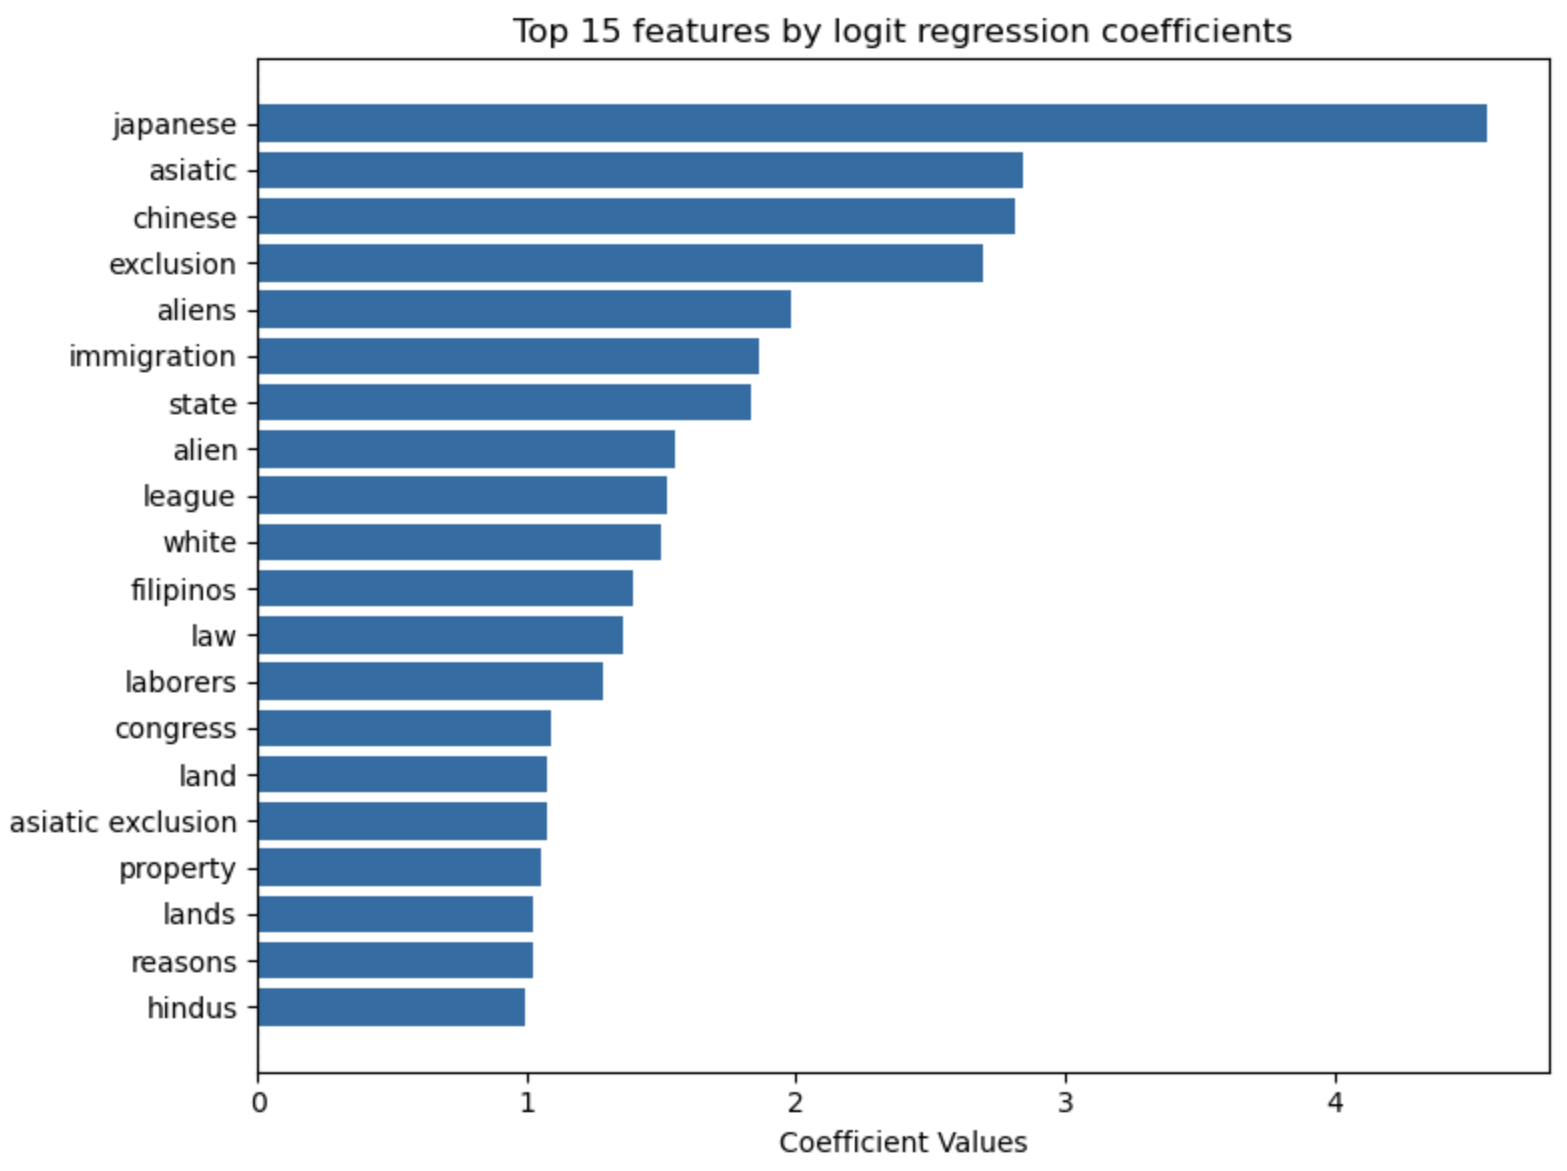
\includegraphics[width=0.75\textwidth]{top15w.png}
	\caption{Top 15 Nativist Indicators}
	\label{fig:top15}
\end{figure}

The logistic regression models demonstrated a relatively strong ability to differentiate nativist articles. Training the model on \textit{75\%} of my handcodes and using the remaining \textit{25\%} for validation, the logistic regression model performed best among the models, with an overall accuracy of \textit{0.86}. Figure \ref{fig:classrep} reports crucial accuracy metrics for both classes. Class 0 (non-nativist) has a precision of 91\% and a recall of 88\%, indicating that the model makes highly reliable predictions for this class. For class 1 (nativist), the model scores a precision of 76\% and a recall of 81\%. When corroborated by the confusion matrix in Figure \ref{fig:conmat}, this indicates that nativist predictions may contain more false positives. The model was trained on sentences, then applied to full articles; robustness checks found no systematic difference in classification confidence between the two.

\begin{figure}[H]
	\centering
	\resizebox*{1\textwidth}{!}{%
		\begin{tabular}{ |p{3cm}||p{3cm} |p{3cm} |p{3cm} |p{3cm} |   }
			\hline
			Class& Precision & Recall & F1-Score &Support \\
			\hline
			0   & 0.91    &0.88&   0.90 & 207 \\
			1 &   0.76  & 0.81   & 0.79 & 95 \\
			\hline
		\end{tabular}
	}
	\caption{Classification Report}
	\label{fig:classrep}
\end{figure}
\vspace*{0.5cm}

\begin{figure}[H]
	\centering
	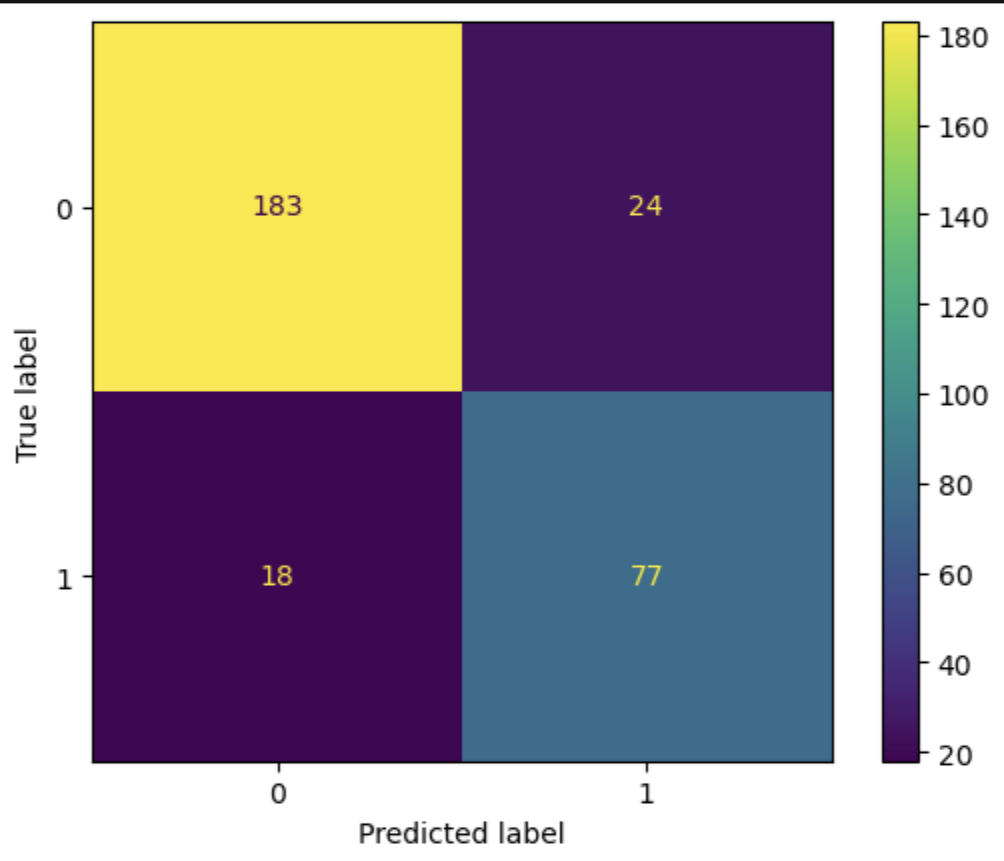
\includegraphics[width=0.75\textwidth]{confmat.png}
	\caption{Confusion Matrix}
	\label{fig:conmat}
\end{figure}

I included a robustness check after training my model to determine whether sentences would translate well into full articles. The checks included creating a sample, running six spot checks on my classified corpus, and comparing the confidence of each model prediction with the same portion of my corpus, which was split into sentences and then passed to the model for classification. Maintaining article-level text was crucial for readability and to ensure the text was not context-free, especially when conducting close readings of nativist articles. All predictions were over \textit{50\%} and ranged from about \textit{55\%} to \textit{85\%}. The absence of systematic differences in classification confidence confirms that the article-level nativist estimates are not distorted by the use of sentences in training design.
 

%=============================================================
\section*{IV. Analysis}
\addcontentsline{toc}{section}{IV. Analysis}
%=============================================================
\subsection*{A. General Analysis}
\addcontentsline{toc}{subsection}{A. General Analysis}

Analyzing general, yearly trends of nativism shows a decrease in nativist rhetoric, consistent with the theorized decay of the mechanism over time. I plotted the average nativist text per year and used a Simple Moving Average (SMA), averaging over the past $n$ periods ($n=6$) to filter out noise and capture general trends. Figure \ref{fig:nat} illustrates general trends in nativist rhetoric, indicating a consistent presence of nativist sentiment over the intervening decades, despite gaps in the literature. The overall decrease in nativist sentiment confirms the theoretical prediction that SMU would progressively erode nativist mobilization. Nativism remained consistently low around 1960, confirming that California's embrace of SMU began earlier than its formal theorization. The linear regression corroborates this, indicating that time is a statistically significant variable and that an increase in years is associated with a decrease in nativism. The largest yearly spikes in nativist sentiment occurred in 1908, 1926, and 1929-- which is slightly different when looking at monthly averages--, all of which largely align with major political and economic events, indicating that it is not merely steady immigration rates or unemployment that trigger these spikes, but rather exogenous shocks.
\begin{figure}[H]
	\centering
	\includegraphics[width=\textwidth]{natm1.pdf}
	\caption{Yearly Nativist Sentiment: 1900-1988}
	\label{fig:nat}
\end{figure}

When plotting Figure \ref{fig:nat} with various time series that reflect both economic and cultural threats, I find that, in isolation, they are poor predictors of nativist sentiment, consistent with theoretical expectations. In the sixties, nativist rhetoric increased modestly alongside immigration rates, at a substantially lower magnitude than in prior decades, then underwent a full reversal by the late seventies, with nativist rhetoric decreasing as immigration rates increased, further aligning with initial theoretical expectations derived from the shift to SMU. However, after running an Engle-Granger Cointegration test (See Appendix B for results), I failed to reject the null hypothesis that the two series are not cointegrated and do not share a long-term equilibrium relationship. This confirms that there is a different underlying process driving nativist sentiment, rather than immigration rates alone– confirmed by theoretical expectations of political opportunity and boundary-making crucial to spikes in nativism.
\begin{figure}[H]
	\centering
	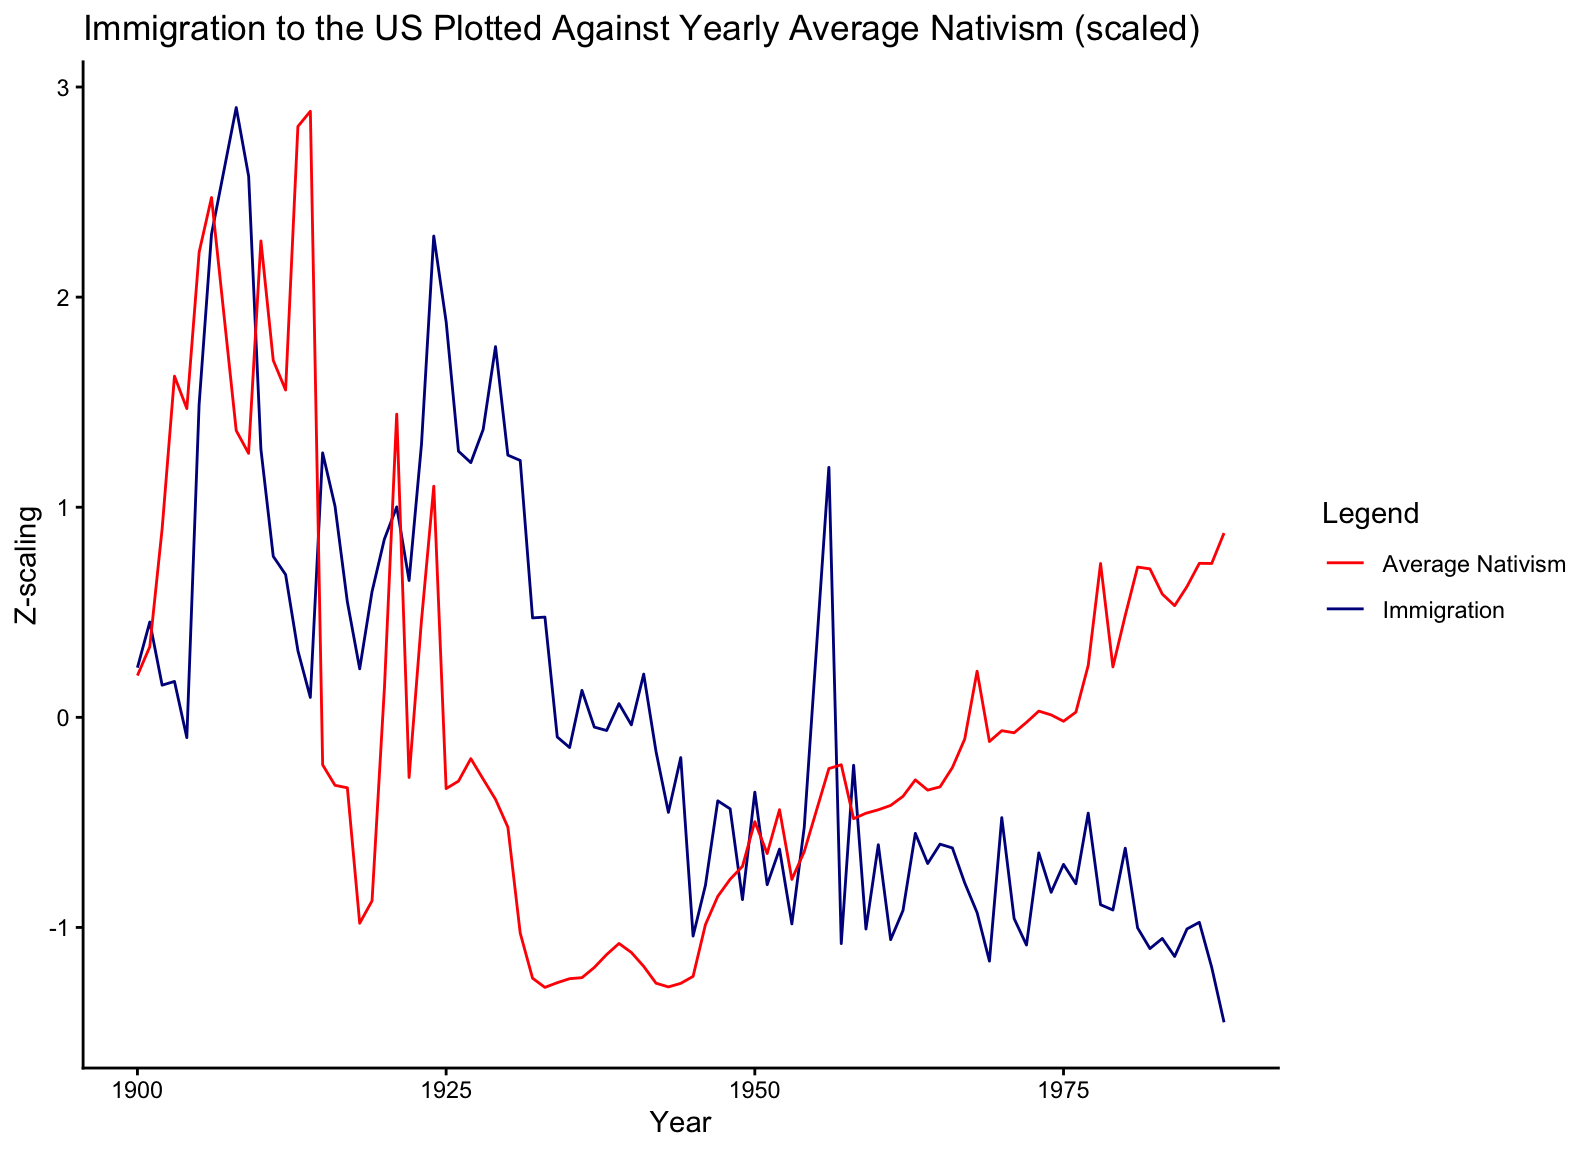
\includegraphics[width=\textwidth]{finalin.png}
	\caption{Yearly Nativism and Immigration Rate}
	\label{fig:Immnat}
\end{figure}

Plotting the time series alongside the percentage unemployment rate amongst the civilian labor force, I found no visually consistent relationship between unemployment and nativist sentiment. Through a visual inspection, there does not appear to be a viable relationship between the two series, as there was with immigration rates. When running another Engle-Granger Cointegration test(See Appendix B for results), I once again failed to reject the null hypothesis that the series are not cointegrated and unemployement does not account for long-term variation in nativist rheotric, confirming theoretical expectations that realistic threats, such as unemployment in isolation, are insufficient to predict nativism. 

\begin{figure}[H]
	\centering
	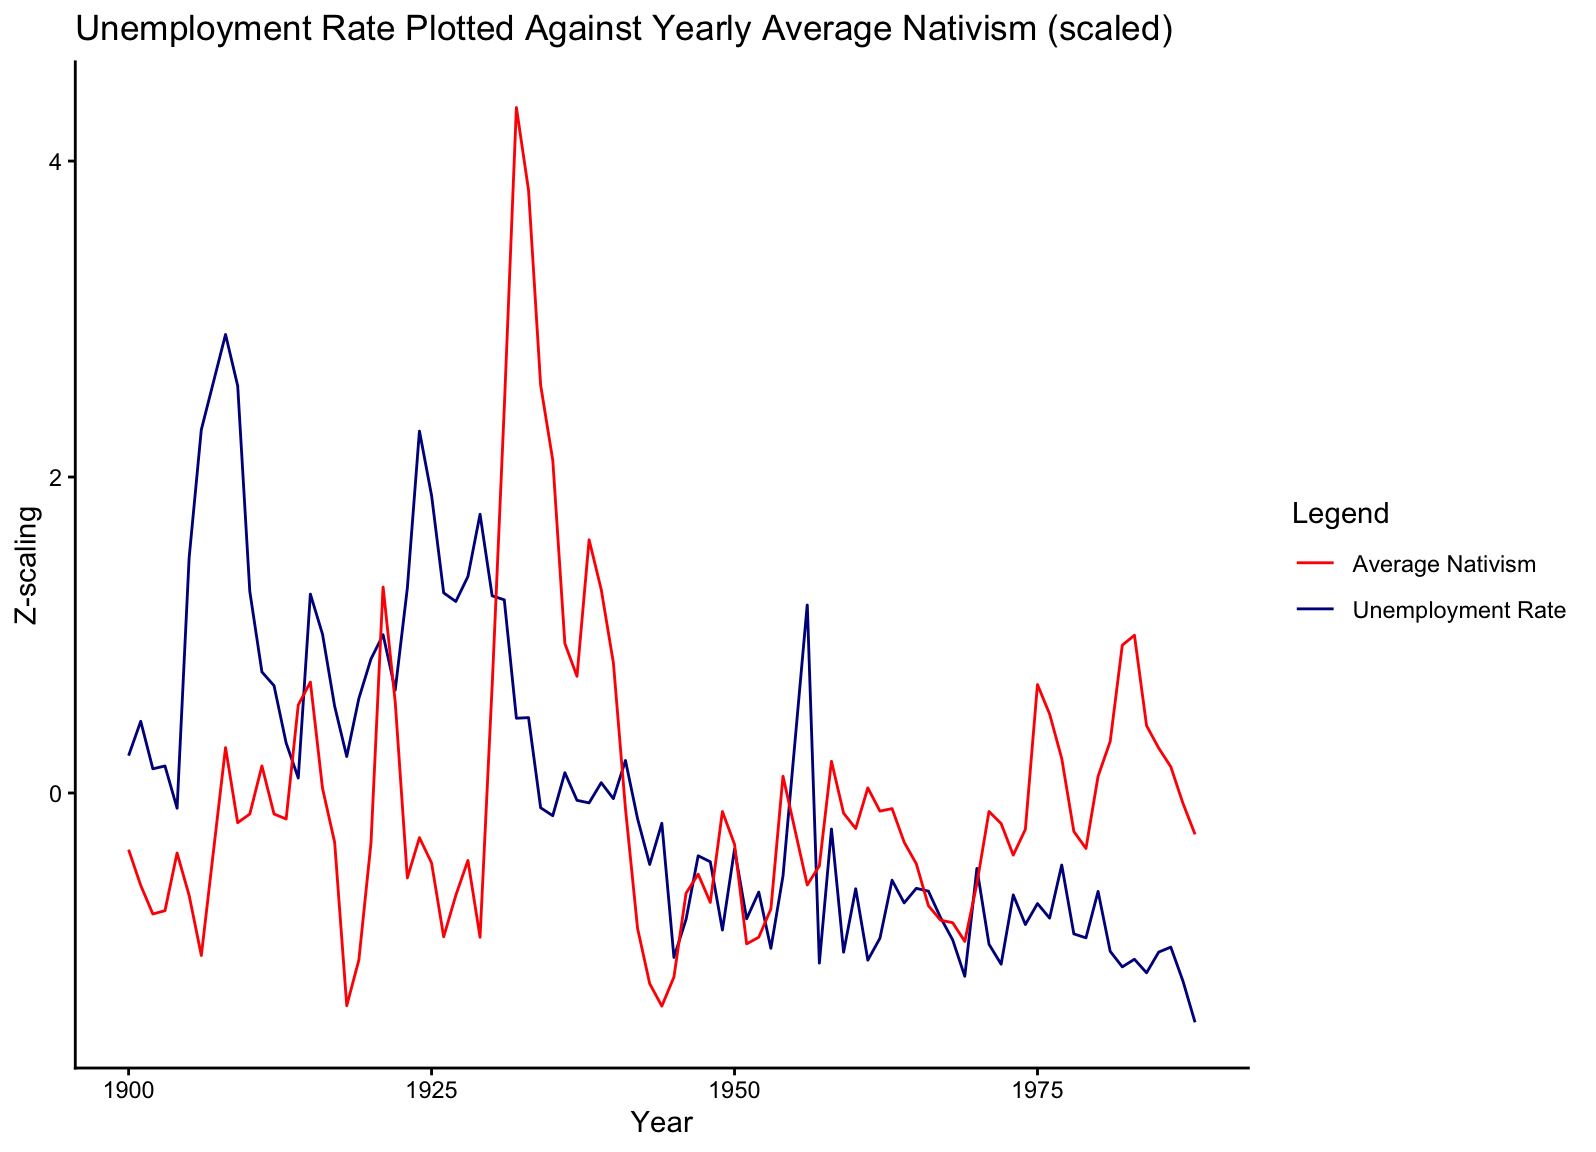
\includegraphics[width=\textwidth]{finalen.png}
	\caption{Yearly Nativism and Unemployment Rates}
	\label{fig:unempnat}
\end{figure}


\subsection*{B. Early Twentieth Century (1900--1930)}
\addcontentsline{toc}{subsection}{B. Early Twentieth Century (1900--1930)}

The early twentieth century most strongly reflects the nativist mechanism with the clearest language of racial threat and economic competition amid ongoing recession, a major world war, and major advancements in the agricultural and industrial sectors. In this period, I found that nativism spiked following the national recession, during times of societal unrest, with clearly identified goals of both racial preservation and lessened economic competition. Unions explicitly blamed immigrants for economic instability and unemployment, without acknowledging corporations' role. This period has the highest overall nativism rates among the decades. The highest monthly nativist spikes occurred in 1909 and 1926, following national economic shocks and occurred within moments of nativist mobilization among local populations, including anti-Asian mob violence.

\begin{figure}[H]
	\centering
	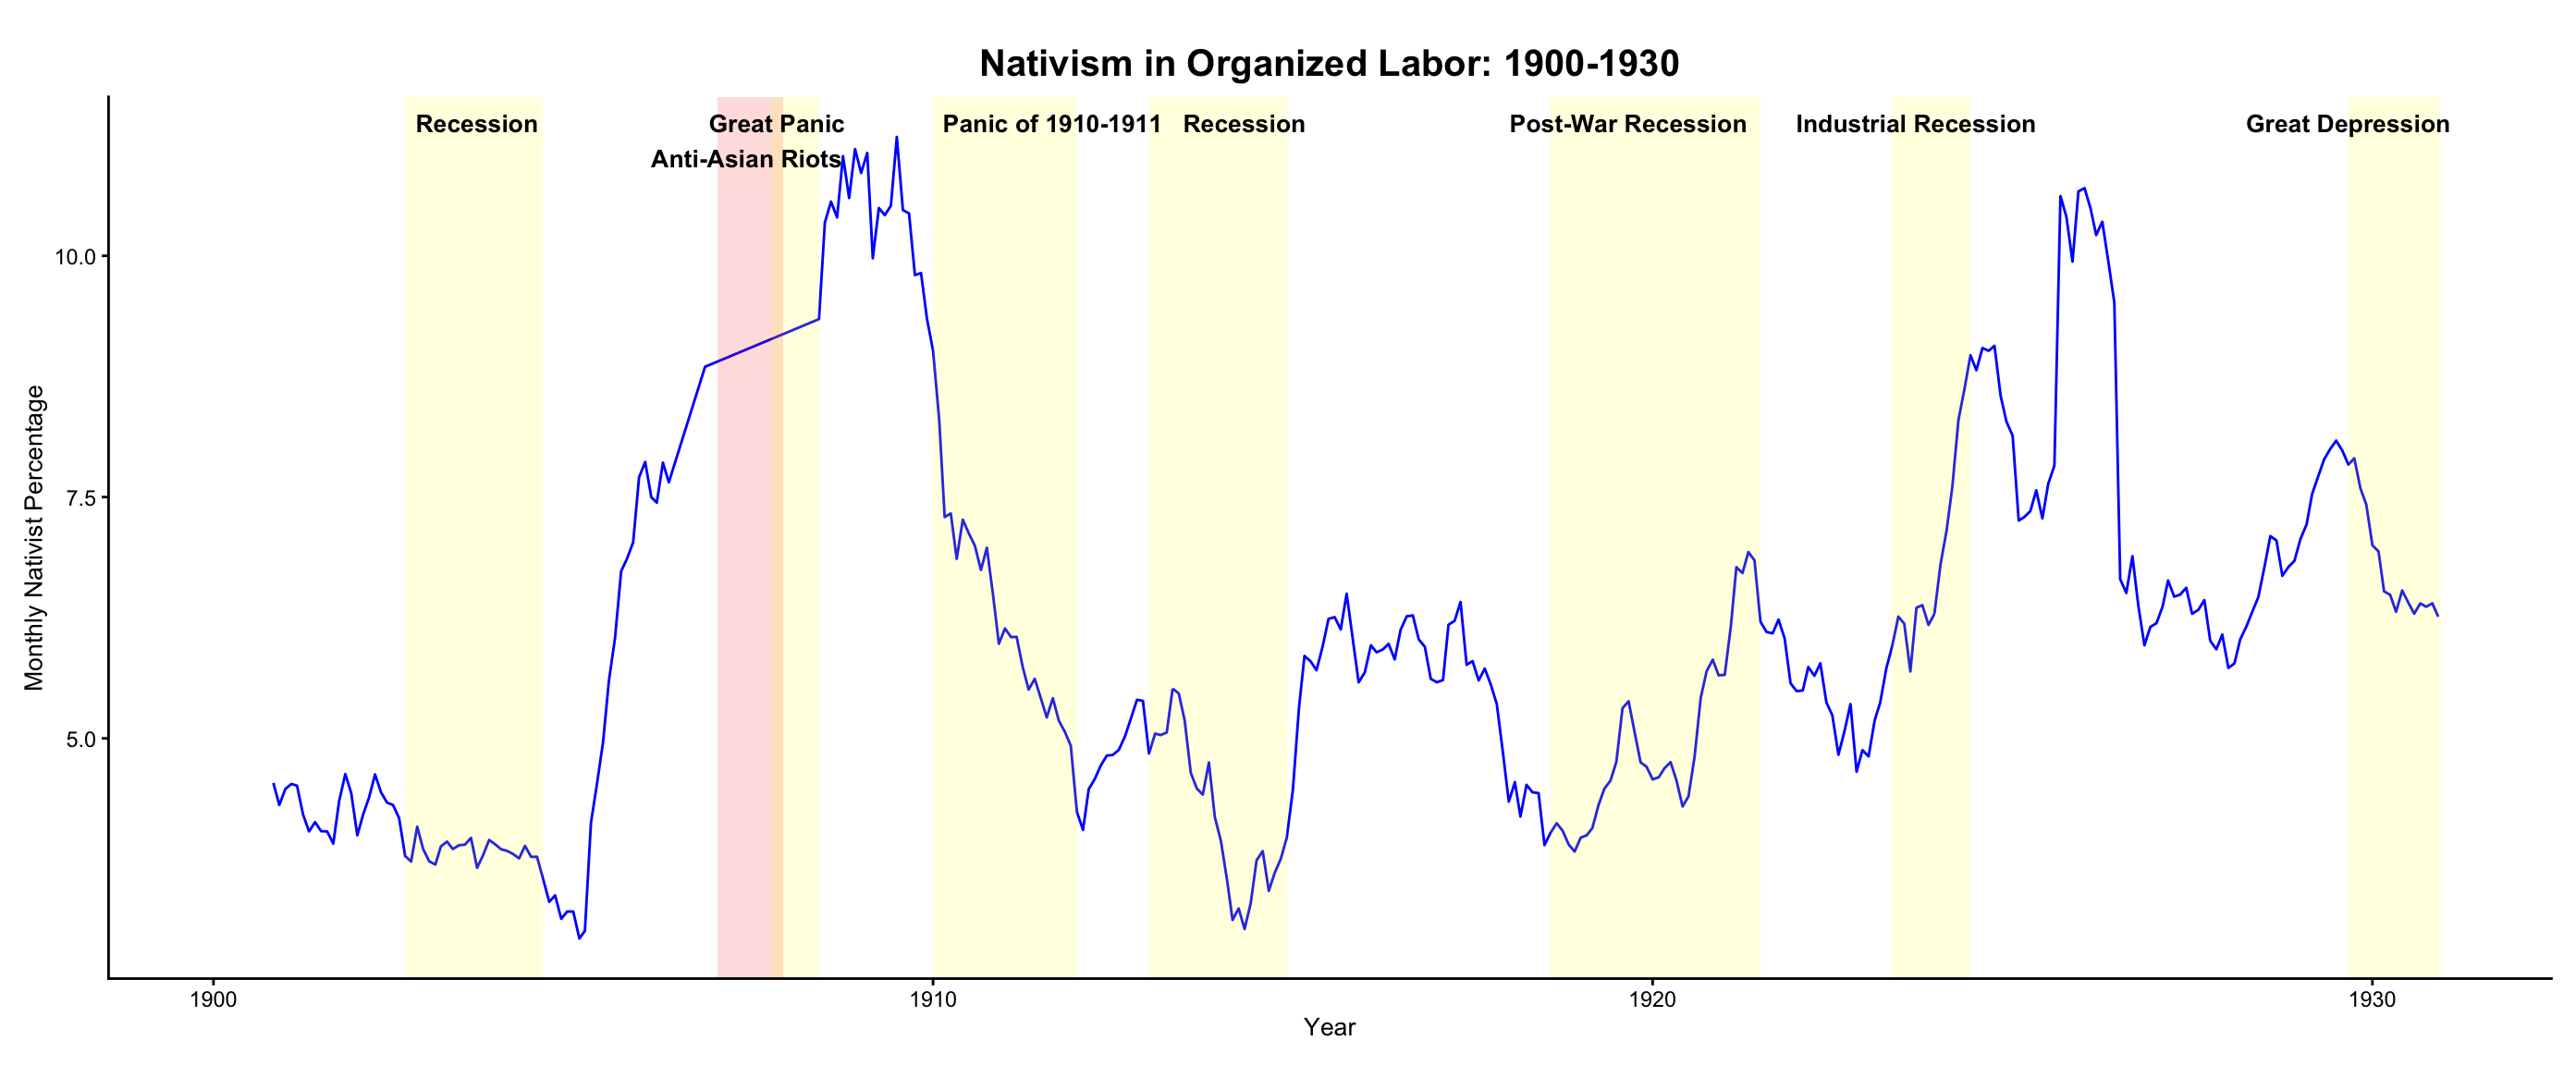
\includegraphics[width=\textwidth]{final00.png}
	\caption{Nativist Sentiment: 1900-1930}
	\label{fig:nat1}
\end{figure}

The first major spike occurred in 1909, following national panic, amid mob-led riots, and rising immigration rates. In 1906, a sharp increase in immigration created an initial sense of tension between immigrant and local populations, which was then exacerbated by the Panic of 1907. The Panic of 1907 is one of the most severe financial crises in the US before the Great Depression, and it began with damage from the 1906 San Francisco earthquake. During the Panic, in the spring, summer, and fall of 1907, there was a series of intense riots in San Francisco, Bellingham, and Vancouver, Canada, that were interconnected uprisings of anti-Asian nativist violence. \footcite{lee_hemispheric_2007} Mobs---including members of the Asiatic Exclusion League---would go into homes and workplaces of Asian immigrants, and destroy property and harm people, with the intention of removing them from their cities. Riots led to an informal agreement between the US and Japan, titled the Gentlemen's Agreement, which aimed to reduce Japanese immigration to the US. \footcite{lee_hemispheric_2007} \textit{Organized Labor} was central to these riots through institutional ties to the Asiatic Exclusion League, which made the paper a vehicle for amplifying the cultural threat to a labor audience; therefore, its coverage reflected and amplified the riots' nativist logic. The convergence of both cultural and economic panic created the necessary political opportunity structure through which boundary-entrepreneurs in \textit{Organized Labor} mobilized nativist frames targeting Asian immigrants. 



Labor unions utilized the conditions of the economic threat and organized mob violence to mobilize in defense of racial preservation and economic interests. In an article titled `An Open Letter to Roosevelt' by H. F. McMahon, written in March 1909 in \textit{Organized Labor}, McMahon states that the ``anti-jap laundry league'' was formed, ``not until the Japanese had increased in the laundry industry over \textit{100 percent} since the fire of 1906. Presently, similar conditions existed in other localities throughout the State---the Japanese were prospering while large numbers of our white men and women were walking the streets in idleness.''\footcite{mcmahon_open_1909} The 1906 earthquake/fire was a precursor to the Great Panic; in this context, the author invokes the conditions created by economic threat and then builds upon them to mobilize not only their economic but also their cultural concerns. The article continues that ``this crusade against the immigration and competition of the Asiatic is not, Mr. President, merely an issue of racial prejudice, but it is unquestionably an issue of racial preservation,'' and then explains that the ``Japanese have an inferior standard of living that handicaps the white man and woman in the competitive race for subsistence.'' \footcite{mcmahon_open_1909} By amplifying racial preservation, the article is essentially selecting the frame most useful for mobilizing against immigration, consistent with Wimmer's argument that boundary-making actors select ethnic frames that are advantageous rather than objective threat metrics. The rhetorical sequence in this article demonstrates the mechanism by which nativism is driven: increased immigration, national economic shock, followed by a mobilized campaign expressing both a need for racial preservation and economic benefit.

The next largest increase in nativism is situated between two economic recessions in 1926, which featured growing economic competition between unions and Mexican workers and a targeted state-sponsored federal campaign against the new immigrant population. The recession in 1923, before the spike in nativism, was relatively brief and, compared with the pre-WWI recessions, considered mild, with real Gross National Product falling by only roughly \textit{4\%}. During this recession period, the Johnson-Reed Act of 1924 went into effect, essentially leading to the full exclusion of Japanese immigrants, which was highly motivated by racial preservation. As a result, employers recruited Mexican labor, leading to growth in the Mexican immigrant population and a growing sense of competition with union members, further exemplified by recurring national recessions. \footcite{gomez_rhetorics_2024} The AFL expressed that Mexican labor is ``cheap peon labor'' that is essentially driving down wages and replacing Americans.\footcite{reisler_always_1976} Despite the economic recession being classified as mild, when coupled with the immigration anxieties created by the campaign for the Johnson-Reed Act and the growing immigrant population, these conditions were sufficient for nativist sentiment to grow. This initial economic rift then enabled boundary-making actors to induce cultural panic, which was institutionalized through state-sponsored campaigns such as the 1925 study by the Secretary of Labor on Mexican immigration. This study concluded that there was a ``new problem'' and that research was needed to restrict it.\footcite{calderon-zaks_debated_2011} This was furthered by institutional channels when Senator John Box introduced a bill to Congress for the exclusion of Mexicans.\footcite{calderon-zaks_debated_2011} Through state-sponsored legislation and the legitimization of the economic and cultural panic, unions then had a political opportunity through which they could mobilize against Mexican immigrants. 

Labor unions during this spike shifted their nativist mobilization from Asian immigrants to Mexican immigrants, using similar language and motivations to mobilize against the most useful ethnic target in the current political and economic conditions. There is a reaffirmation of Asian exclusion in an article on the 16th of January 1926, titled ``Shortridge Ired by S.F.\ Chinese Plea for Alien Law Change.'' The article explained, ``The exclusion provision is to prevent a multiplication of Orientals in this country. The Orientals are not assimilable with Americans, as are other racial groups; to permit them to increase in numbers, it would be encouraging an eventual race conflict.'' This demonstrates unions' reaffirmation of the unassimilable nature of Asian immigrants and their desire for racial preservation---highlighting unions' maintenance of previous nativist boundaries whilst creating new ones, highlighting nativism’s cumulative and institutional nature, rather than a simple reaction to ongoing conditions. A different article, amidst the spike titled \textit{Congressman Flaherty Launches Campaign to Stop Mexican Invasion of U. S.} the author explains ``Morally as well as economically, their presence is detrimental to the nation\ldots the majority of prisoners are Mexicans\ldots one-half of the money given for charity in Los Angeles is expended on the indigent Mexican population'' and also highlights ``These Mexican laborers are doing work that otherwise would be done by American citizens. The Mexicans do not, as a rule, become American citizens.'' \footcite{ely_congressman_1925} The core principles of preservation and economic stability continue to serve as central motivating factors for their nativist advocacy. The difference lies in the shift from Asian to Mexican immigrants and the boundary of exclusion, which demonstrates how their mobilization is constructed alongside dominant cultural targets. The boundary is no longer whiteness explicitly, but citizenship and Americanness. The shift towards citizenship reflects the fluid nature of boundary-making, given that Americans viewed Mexicans as white given a strict black-white binary; therefore, they required a different basis for othering Mexican immigrants beyond racial exclusion in the post-Johnson-Reed political context. \footcite{menchaca_recovering_2001} Labor unions' amplification and construction of citizenship-based exclusion in place of racial boundaries is clear evidence that target selection followed a strategic opportunity rather than an objective threat. 
\newpage


\subsection*{C. Middle Decades (1930--1970)}
\addcontentsline{toc}{subsection}{C. Middle Decades (1930--1970)}

The next period, from 1930 to 1970, is crucial, as it reaffirms the patterns of nativist sentiment whilst demonstrating both weaknesses in the theory and a decay in the mechanism. Figure \ref{fig:nat2} demonstrates that overall nativist sentiment decreased greatly within the middle decades and remained relatively low throughout the period. However, there were significant fluctuations throughout, particularly in 1931, 1941, and 1954.  In the first spike around 1931, during the Great Depression, the language of the 1926 spike persisted, with increased emphasis on economic stability over racial preservation. Compared to earlier spikes, given the conditions of the depression, there was an overemphasis on deportations due to a need for employment and social security. Following this spike, the next increase in 1941 occurred alongside the US entry into WWII. This spike quickly dissipated, ushering in a newfound sense of ethnic unity. Despite economic instability and cultural panic among local communities, nativist sentiment decreased, suggesting a possible confounding variable–state-sponsored unity campaigns. Finally, the last spike occurred in 1954, during the federal funding of ``Operation Wetback,'' coupled with economic recession. Overall, in these decades, there is a waning emphasis on racial preservation, and union members place greater emphasis on blaming corporations than in the previous decade. This is consistent with the theoretical expectation that SMU would progressively decay the racial dimensions of nativism.
\begin{figure}[H]
	\centering
	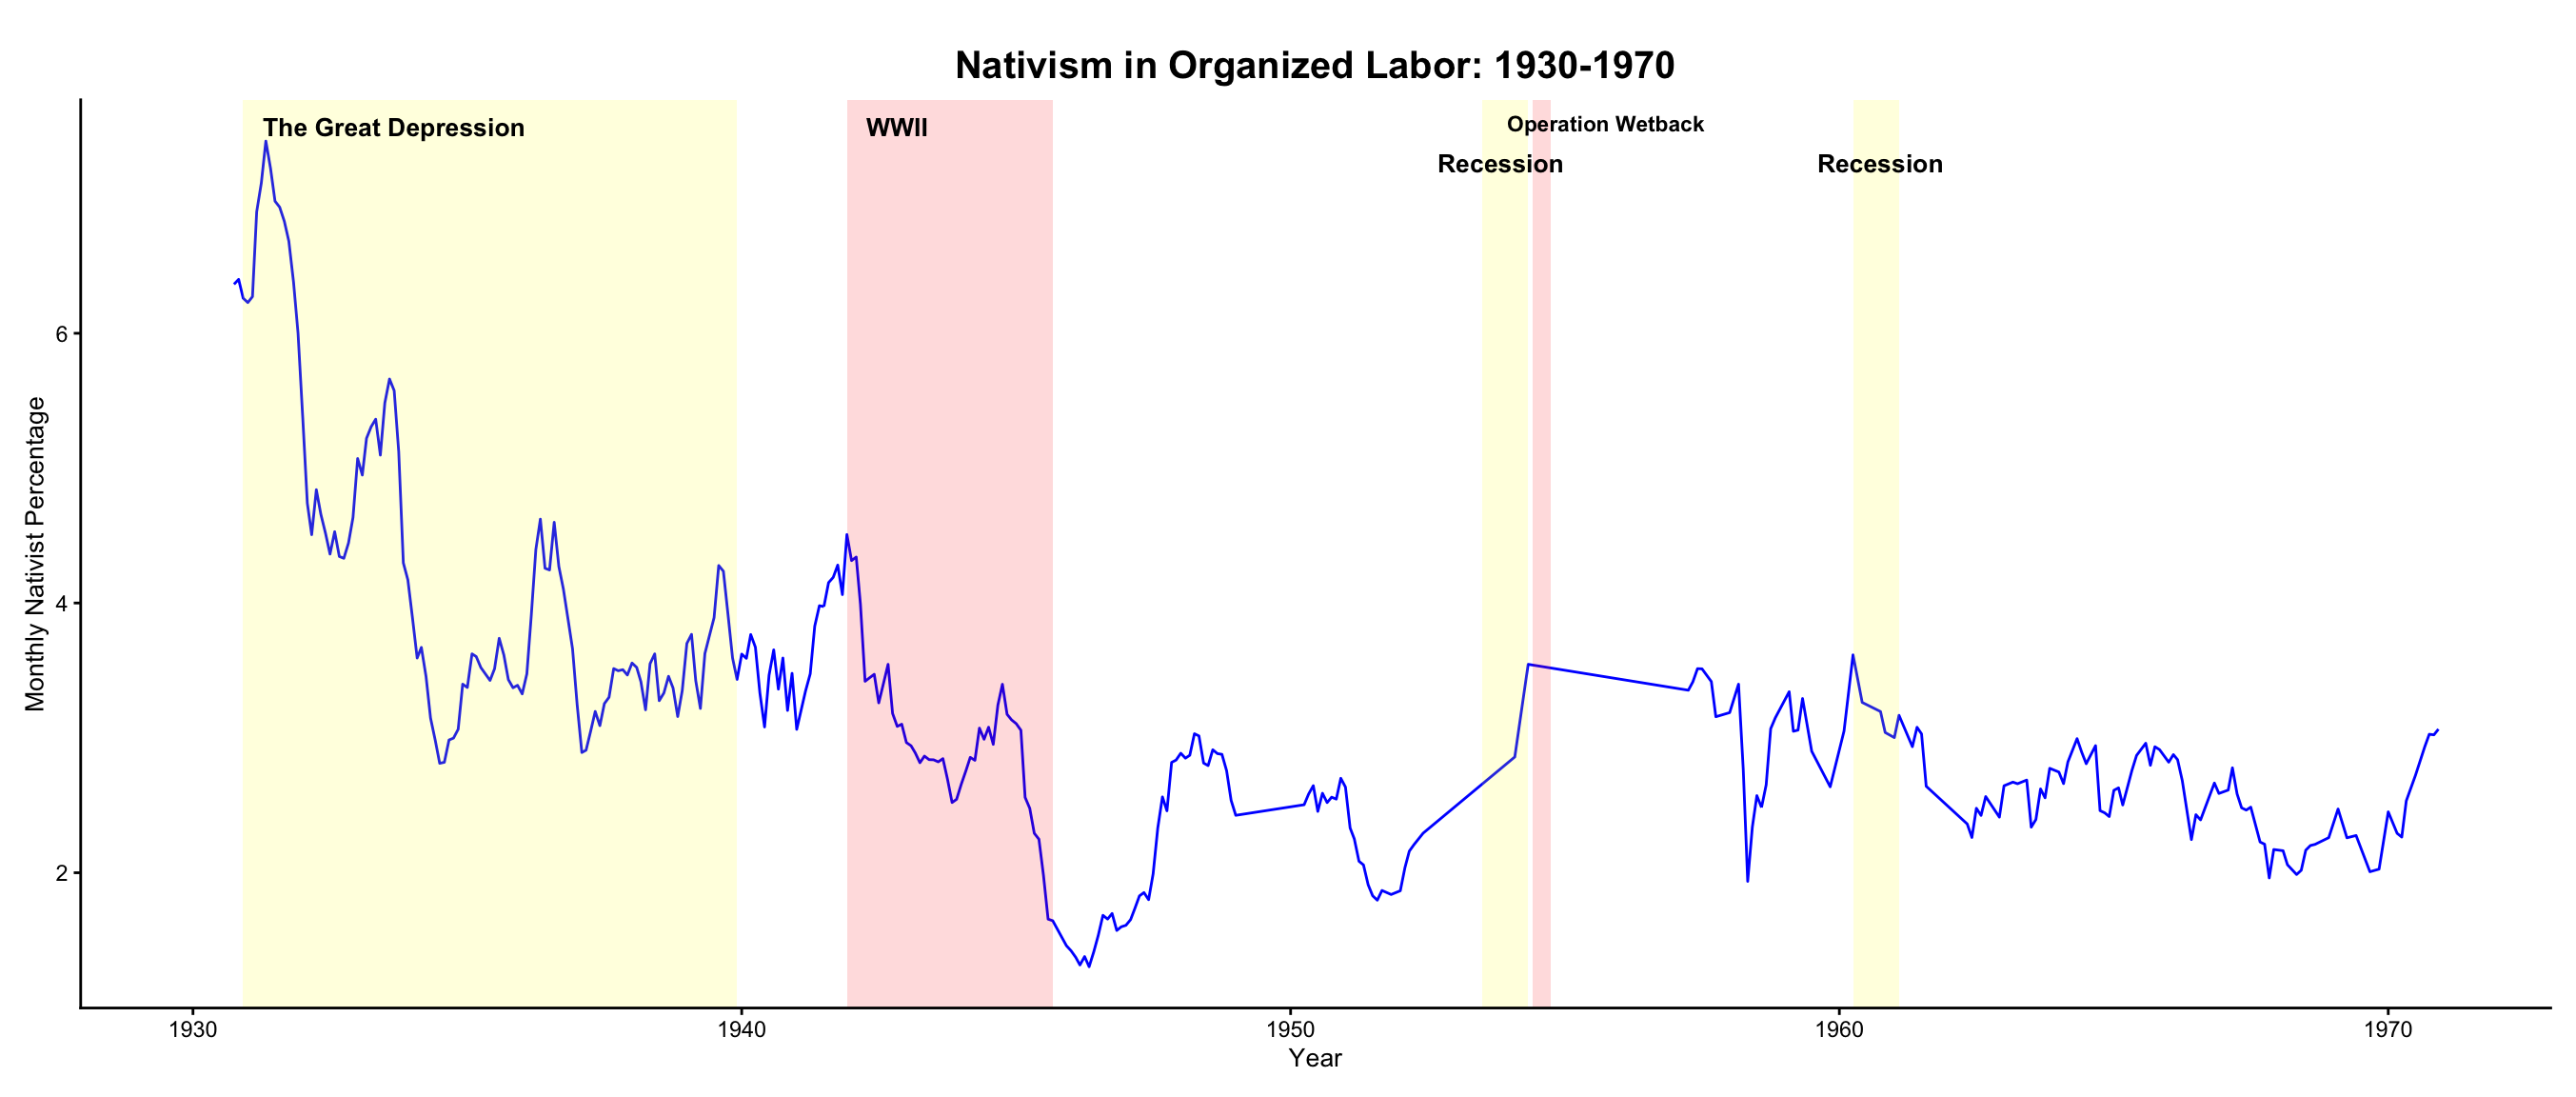
\includegraphics[width=\textwidth]{final30.png}
	\caption{Nativist Sentiment: 1930-1970}
	\label{fig:nat2}
\end{figure}
The spike in 1931 is situated amid the Great Depression, with shifts in perceptions of immigration policy, occuring alongside the federal government's weaponized economic anxiety in the justification of mass deportation. The Great Depression, one of America's worst economic crises, began in 1929 and lasted until about 1939. In the years before the Great Depression, as shown in Figure \ref{fig:Immnat}, overall immigration declined due to the 1924 quotas, but Mexican immigration remained elevated due to employer recruitment. Once the depression hit, the unemployment rate was incredibly high, thereby exacerbating initial economic competition between Mexican workers and union workers. The issue of unemployment thus provided another opportunity for boundary-making actors to cultivate a narrative featuring a growing threat of Mexican immigration amid economic panic, whilst building on earlier rhetoric to isolate and otherize Mexican immigrants. Further national eugenicists' publications began to highlight the financial cost of labor competition and of free clinics for Mexican immigrants, as an unnecessary burden during hardship.\footcite{hubbard_national_2011} The othering of Mexican immigrants began to become institutionalized through deportation campaigns from 1930 to 1933 as a part of Hoover's administrative policy. From the initial shock of the Great Depression, the nativist frames of the 1926 spike created the infrastructure that boundary-making actors reactivated in the depression, shifting legislative restrictions to deportation advocacy.


\textit{Organized Labor}, in particular, responded to the triggers highlighted above by increasing articles encouraging the deportation of Mexican immigrants, centering frames of economic competition, with racial preservation undertones. In one article titled `America Should be Kept White', the author began by highlighting ``despite the fact of widespread unemployment, that there are certain individuals and groups, who are demanding of our government unlimited and unrestricted admittance to this country of Mexican peons.'' \footcite{noauthor_america_1930} One striking difference from anti-Asian nativism and anti-Mexican nativism is that there is some emphasis on attributing blame to recruiters instead of solely to immigrants themselves. This shift reflects a strategic framing choice made during the Depression era, emphasizing blame on employers as well as immigrants, even as working-class people as a whole experienced exploitation, a shift that proved advantageous. The article continues that the issue is ``\ldots more crime is to be found where labor is cheap, that disease and filth abounds among the poorly paid workers, and that all charitable institutions are taxed to capacity, administering relief and assistance\ldots''  \footcite{noauthor_america_1930} By highlighting disease and filth, alongside the scarcity and declining accessibility of relief organizations, unions demonstrate that their goal of reduced economic competition can benefit all Americans. Moreover, the title advocating for keeping America white suggests a desire for racial and cultural preservation. Still, through the construction of America’s situation and the types of threats posed to Americans, economic competition had taken precedence. Another article titled ``DEPORTATIONS NOW EXCEED IMMIGRATION Exodus Is Held to Help Relieve Unemployment`` quotes the words of the Secretary of Labor stating: ```I'm going after every evader of our alien laws, regardless of nationality, creed or color, because I hold the belief that persons who have no right to be here should give their places to Americans\dots.'' \footcite{noauthor_deportations_1931} Through the amplification of Doak’s words, \textit{Organized Labor} demonstrates its motivation for supporting deportations, highlighting passages that stress anxieties about economic framing rather than explicit racial exclusion, indicating that unions intentionally mobilized during the economic conditions of the Great Depression to strengthen their mobilization. The citizenship frame utilized by Doak and reproduced approvingly by \textit{Organized Labor} demonstrates that the nativist objective of racial preservation endures. Still, it is now emphasized through civic rather than racial language. The 1931 example confirms that, as the target and rhetorical frame shift, the causal chain of realistic and symbolic threats that creates a political opportunity for boundary-making remains. However, the lower magnitude of the 1931 spike compared with those of 1909 and 1926, despite worse economic conditions, provides evidence of the mechanism's early decay.

The second-largest peak in the middle decade occurred in 1941, with a \textit{4.5\%} spike, coinciding with the bombing of Pearl Harbor and a slowly recovering economy. One important observation is that following the 1931 spike, the rates of nativist rhetoric subsided, with peaks falling from \textit{10\%} to about \textit{4\%}. In 1941, only two years after the Great Depression ended and as WWII began, the American economy was still recovering; about \textit{10\%} of the workforce was unemployed, which led America to diversify its labor force and to require high wartime production to meet Americans' economic needs.\footcite{daniels_immigration_2006} This initial importation of foreign labor, primarily from Mexico, amid a recovering economy and high unemployment, was met with anger and rejection. Although this was not a recognized national recession, it did cause a moment of economic shock and panic. Further, this period experienced a strong sense of cultural panic, driven by public paranoia discussed in \textit{Panic Politics in the US West Coast} around 1942, fueled by rumors that Japanese Americans were aiding enemies, cementing fear and suspicions amongst the public.\footcite{berman_panic_nodate} Despite moments of panic, Richard W. Steele argued that there was no generation of nativism during the Second World War as there was with the first, given the presence of state-sponsored unifying campaigns. \footcite{steele_war_1989} America was not anti-racist, but wartime emphasis on racial solidarity had a profound impact on negating the causal mechanism that spiked nativist sentiment, despite high unemployment rates and cultural panic.


Labor unions' initial nativist response subsided and was reversed amid wartime emphasis on unity and prevailing political conditions, rendering nativist boundary construction unviable and costly. In the earlier months of 1941, \textit{Organized Labor} published an article titled 'PETITION TO IMPORT ALIEN LABOR INTO STATE SHOULD BE DENIED' arguing against the importation of foreign labor: ``\ldots to exploit the workers of our neighboring country by working them at substandard wages. `We also consider this as an attempt to flood our country with cheap foreign labor while thousands of our citizens are unemployed, anxious, and available for work at decent wages.''' \footcite{noauthor_petition_1941} By highlighting the exploitation of Mexican workers, the article no longer blames immigrants as the sole cause of poor economic conditions, but there is a growing willingness to blame corporate greed. There is still othering through the portrayal of ``our own'' against ``cheap foreign'' labor, stating that continued nativist sentiment was driven by economic competition. A year later, in June of 1942, they published an article titled ``Importation of Mexican Farm Laborers into California Vital Necessity'' in which they report that the Department of Labor and Agriculture is arguing that there is a ``labor shortage with which farmers of this state are faced. That week, the report covered 74,000 people engaged in seasonal farm work. In the previous week, farmers had a shortage of 21,000 workers, whereas in the week ending.''\footcite{noauthor_importation_1942} Compared with previous articles, there is no use of racialized othering in reference to immigrants, no emphasis on protecting American white labor, and the article reports the measure neutrally. Despite economic hardship and cultural panic, state-sponsored attempts to unify citizens during wartime negated the causal mechanism's effect. This disruption confirms that the mechanism is contingent on political context. Specifically, state-sponsored ideological campaigns can negate spikes in nativist sentiment despite the present cultural and economic threat. This disruption to the causal chain is the first clear case of nativist decay, foreshadowing the post-1960s decay, given that the average nativist sentiment continues to shrink under the same conditions that previously produced major spikes. 

Another rise in nativism in the middle decade comes in 1954 during the launch of Operation Wetback, and economic recovery; importantly, though, unions exhibit a discernible shift towards more class-conscious, neutral positions compared to earlier decades. During the recession of 1953--54, following the end of the Korean War, US industrial production declined by \textit{10\%}, and the postwar unemployment rate of around \textit{2.3\%} rose to about \textit{6.1\%} in late 1954.\footcite{lovasy_prices_1956} Alongside this downturn, Operation Wetback was launched by the US Border Patrol in May of 1954, the same month as the spike, as an attempt to respond to the ``crisis'' of undocumented Mexican immigration caused by the Bracero Program.\footcite{hernandez_crimes_2006} The Bracero Program was an initiative launched during WWII as a way of cyclically importing Mexican labor to address shortages caused by Japanese internment and enlistment.\footcite{hernandez_crimes_2006} Agencies such as Border Patrol and other federal actors constructed a symbolic threat– framing Mexican immigrants as an invasion– which institutionalized the anti-Mexican nativist boundary that boundary entrepreneurs began constructing in the thirties.  For example, the Commissioner of Immigration and Naturalization and the U.S. President's Commission on Migratory Labor referred to the influx of Mexican immigration as a great invasion.\footcite{brinkman_working_2009} Despite the institutionalization of the Mexican threat narrative and intensifying labor competition, the mechanism’s intensity is lower than in previous periods, consistent with the decay argument as the racialized dimension of nativist mobilizations erodes through class-conscious solidarity. 

Articles from \textit{Organized Labor} feature a continued decay in the mechanism, as nativist mobilizations became less racialized and cemented the importance of corporate greed in producing competition rather than immigrants themselves. On the 16th of April 1954, in an article titled “WETBACKS GET BETTER CARE THAN MIGRANTS”, the article quotes Rep. Harold Cooley explaining that Mexican migrants are provided sickness, burial, and accident insurance while “...our own migratory workers who go from one state to another, with their wives and little children. We should give serious consideration to our own migratory labor problem—and to the unemployment problem of our own country.’ “ \footcite{noauthor_wetbacks_1954}  In the same publication, another article titled ‘How Jobless Figures Are Juggled’ explains that “...the continuing challenge to California farm labor embodied in the recruitment of wetback labor by the big farm corporations…” unions have decentered blame from immigrants onto corporations more explicitly than previous articles, consistent with an embrace of SMU. \footcite{noauthor_survey_1954} This perspective is still nativist and thus otherizes immigrants; however, the racialized dimension that was clear prior has become less of the main contention. There is no emphasis on protecting American culture and traditions; instead, there is an emphasis on protecting economic stability and social security. The disappearance of the language of cultural preservation from the 1954 articles, despite rampant invasion rhetoric, confirms that the cultural dimension has been eroded, leaving the economic dimension present yet indistinguishable from class-based SMU organizing.



\subsection*{D. 1970--1988 Period}
\addcontentsline{toc}{subsection}{D. 1970--1988 Period}


Nativism in \textit{Organized Labor} had largely dissipated in this period, no longer achieving spikes in nativist sentiment as in the previous decade, and the language of racial preservation was largely absent from the corpus. Many academics, such as George J. Sanchez and Dina Gavrilos, argue that there was a return to nativism among the general public in the late 20th century. \footcites{gavrilos_becoming_2010}{sanchez_face_1997}  However, there are no longer major escalations in nativist sentiment despite the presence of economic and symbolic threats as well as ongoing campaigns targeting immigrants. Major nativist legislative actions include the Immigration Reform and Control Act of 1986, which enacted provisions that criminalized employers knowingly hiring undocumented immigrants and increased resources for the US Border Patrol to prevent immigration through deterrence, indicating that there was a societal return and reignition of nativist sentiment.  As stated in the methodology section, this era contains few real nativist articles; the algorithm's classification of international competition as nativism reflects the linguistic similarity to the training data rather than genuine nativism. This behavior confirms the decay argument, given that the language then used to create nativist boundaries now merely reflects international competition. There were no longer intentional, targeted campaigns aimed at restricting immigration to the United States despite the presence of input conditions such as national economic recession and nativist cultural campaigns. This is a result of the SMU mechanism becoming fully realized, as Bay Area unions have fully embraced a form of class-based solidarity campaigns. 

\begin{figure}[H]
	\centering
	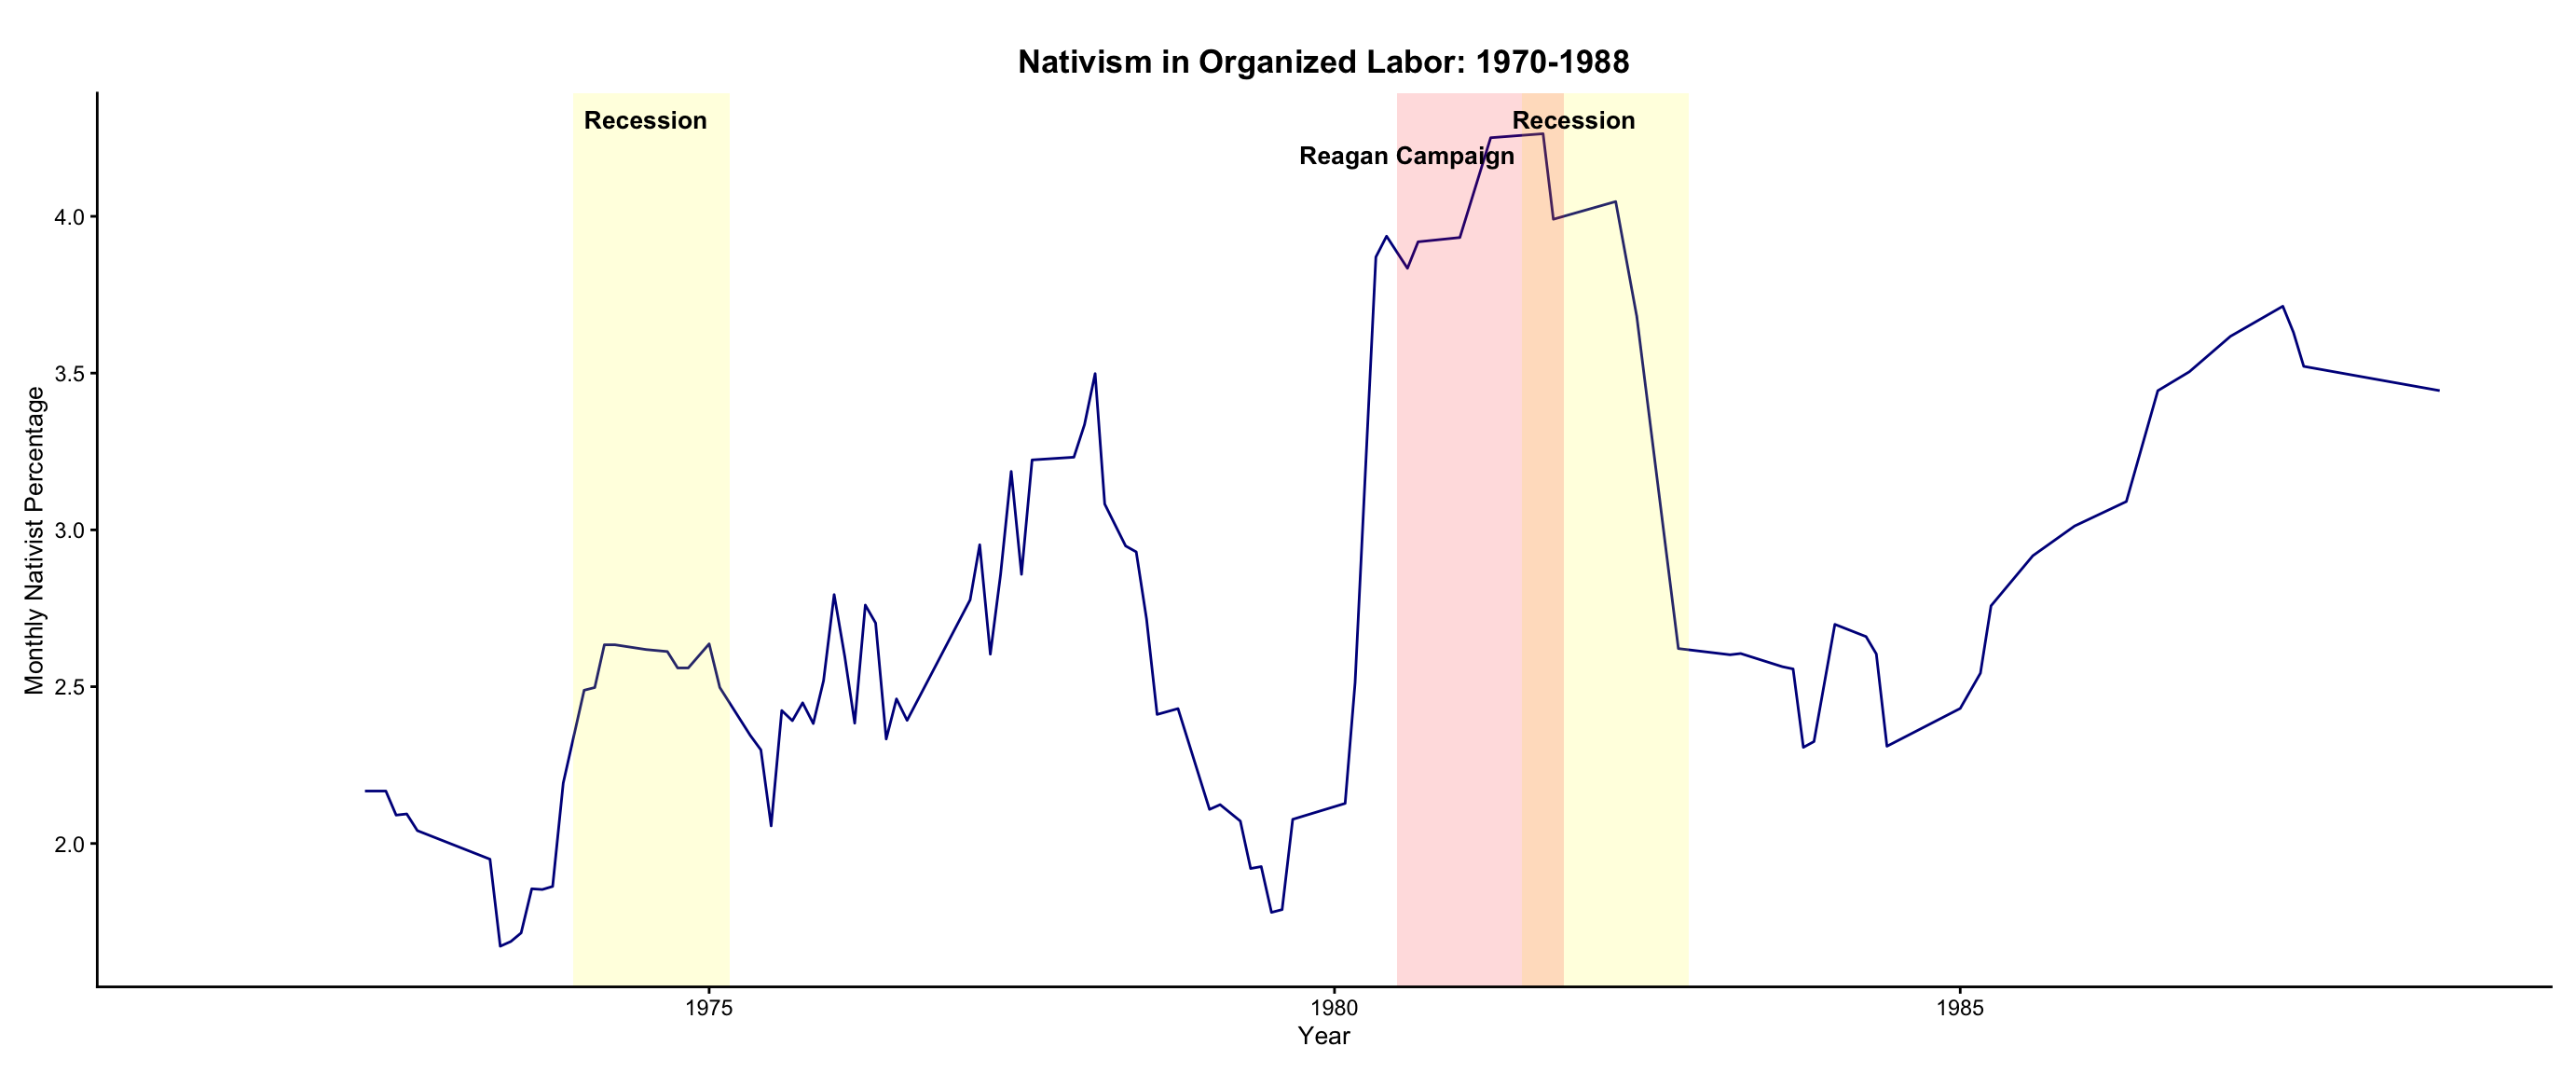
\includegraphics[width=\textwidth]{final70.png}
	\caption{Nativist Sentiment: 1970-1988}
	\label{fig:nat3}
\end{figure}

The biggest spike in the late twentieth century was in 1981, with \textit{4.25 percent} of nativist sentiment, amidst a national recession and increased competition from Japanese companies in the automobile industry.  The recession of 1981 was considered one of the worst recessions since the Great Depression, with an unemployment rate of nearly 11 percent in 1982. The recession induced competition with union workers, generating economic anxiety, particularly in the automobile industry nationally, given the importation of Japanese automobiles and workers. Dana Frank in \textit{Demons in the Parking Lot: Auto Workers, Buy American Campaigns, and the 'Japanese Threat'} argues that there was a revival in "Yellow Peril" racial imagery and nativist sentiment. In addition to racial imagery, there was the murder of Vincent Chin, which occurred as a result of the escalation in the harassment of Asian American workers in autoworker communities. \footcite{frank_where_2003} The national recession, the growing nativist propaganda, and the murder of Vincent Chin all created an escalation of existing ethnic tensions, which were the conditions under which \textit{Organized Labor} was operating. Despite boundary-making attempts and growing economic competition between workers and the Japanese, there was a lack of nativist mobilization of labor unions in the Bay Area.  

In the months before the spike, there were a few articles in which \textit{Organized Labor} mentioned increasing competition from Japanese labor and growing protests. In January of 1981, an article explained: "Carter ends limits on Japanese color TV imports despite labor protests." \footcite{noauthor_economic_1981}This article describes production competitions with the Japanese and rifts with American labor organizations. However, what is notable about this description is that the article lacks the nativist language of racial preservation and othering. Previous articles that discussed economic competition with foreign workers or industries also highlighted the importance of prioritizing white American labor and the inferiority of immigrant labor forces. Amidst the spike in April, the articles that are flagged as nativist describe the intense competition with Japan, particularly in the automotive industry, and the lack of action on behalf of the US government to provide relief for automotive workers; however, once again compared to other unions and the rest of the United States, many of the articles do not target or other Japanese immigrants in the United States. Further, there is no attempt to highlight the superiority of the white American worker. The spike is not a result of semantic nativism but rather of misclassification, as words describing economic competition with Japan were weighted as a nativist indicator in the training data. The semantic shift is itself evidence of decay, given that the vocabulary of nativism has become detached from its exclusionary former function. The complete shift in approach and the absence of nativist sentiment demonstrate how labor unions in the Bay Area embraced SMU and no longer had a trigger for nativist sentiment, despite the causal mechanism's conditions still being present. While the broader rest of society, as seen in legislative campaigns, Ronald Reagan's election, and other labor unions falling into nativist mobilizations, shows this pattern, the same pattern is no longer present in Bay Area unions. This is not to say that by the 80s, Bay Area labor unions were void of racism and xenophobia as a whole; the unions are no longer intentional actors in nativist boundary-making. They are no longer constructing intentional campaigns to bar immigration whilst calling upon racial preservation and economic competition. 

 
%---------------------------------------------------------------------
\section*{V. Conclusion}
\addcontentsline{toc}{section}{V. Conclusion}
%---------------------------------------------------------------------

This research aimed to understand the causes and historical patterns of nativist mobilization amongst Bay Area labor unions, to inform future organizers and academics about historical patterns for prevention, and to provide new avenues of research. This paper argued that Bay Area labor unions' mobilization of nativism went beyond reaction. Rather, it was intentional, carefully constructed, and opportunistic, aimed at achieving racial preservation and reducing economic competition. Objective threat levels did not determine targets of nativist boundary construction, but rather who boundary entrepreneurs found most politically available and institutionally useful at a given moment. Further, this paper found that, contrary to Higham’s argument that nativism will continue to reappear stronger than previous spikes, over time, due to SMU and unions’ embrace of class-based organizing, nativist sentiment decayed. Despite similar input conditions, the mechanism failed to fire spikes as high as previous appearances. The research presented in this paper is crucial amid a time of both growing union activity and white supremacy, as understanding historical patterns and recognizing the active role unions played in the nativist movement are essential to ensuring that unions continue to serve as allies to all marginalized communities, especially immigrants. This dissertation also demonstrates the capabilities of text analysis within historical scholarship to analyze long-term shifts and patterns of political discourse. By combining supervised machine learning with close reading of primary source analysis, I was able to unravel historical patterns and relationships that would be difficult to trace with traditional archival research. There have been many limitations in this paper, including the lack of external validation for the hand-coded articles used to train the model, the small sample size, and the misclassification of later decades. This work is not representative of other regions or countries but rather is specific to the Bay Area. There is substantial work to be done by future academics to examine unions across different regions to determine whether similar patterns of nativist mobilization may appear to those in \textit{Organized Labor}. Future academics should also develop a stronger classification model with more hand-coded data and include an external reliability metric. It remains crucial to continue to interrogate the past of even the most progressive institutions and organizations. 


\appendix

\section*{Appendix A: Supplementary Material}
\begin{figure}[H]
		\centering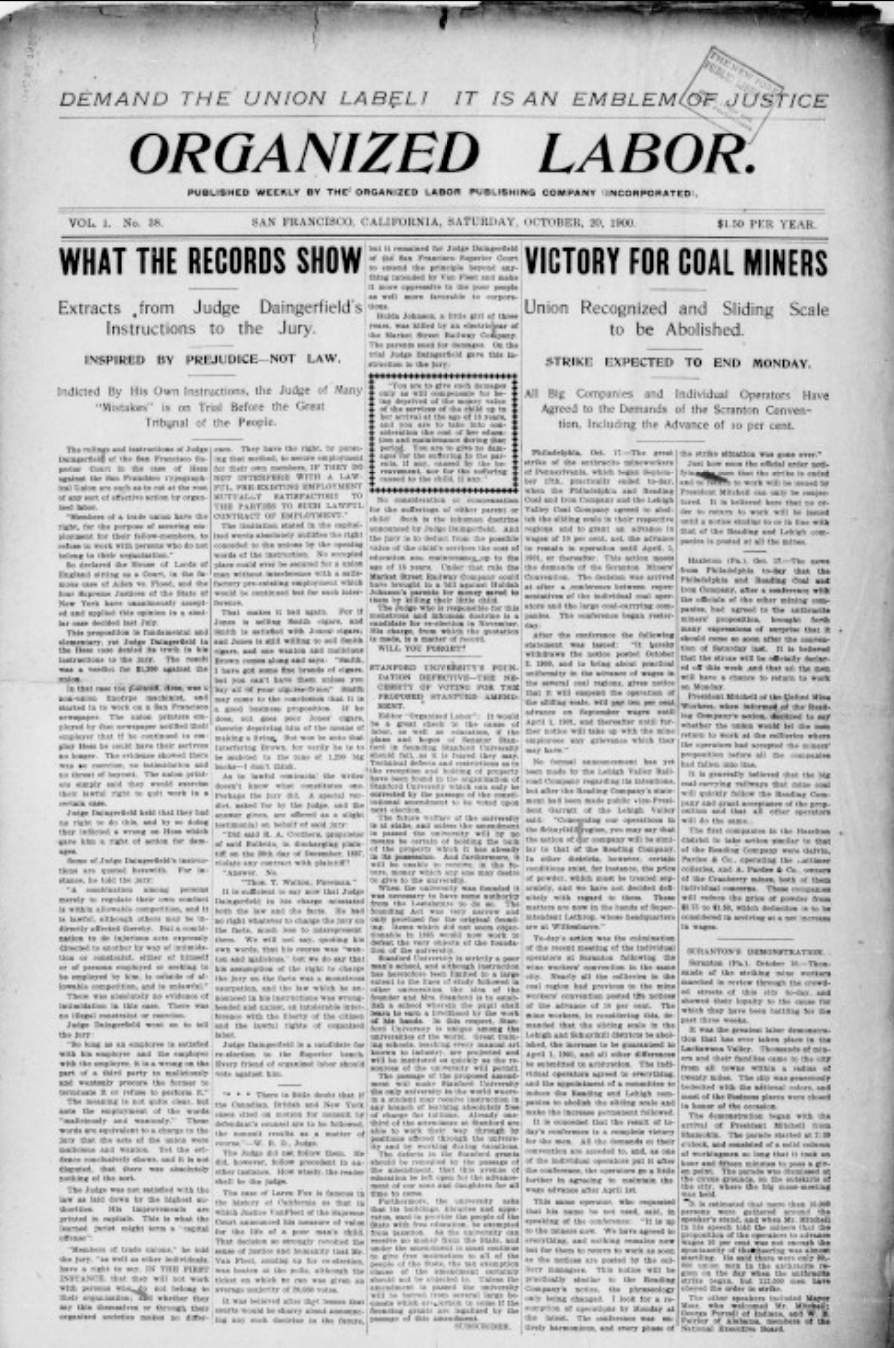
\includegraphics[width=0.75\textwidth]{pagesam.png}
	\caption{Front Cover of Organized Labor Publication - 20 October, 1900}
	\label{fig:sample}
\end{figure}
\section*{Appendix B: Supplementary Tables}

\begin{table}[H] \centering 
	\caption{Engle-Granger Cointegration Test: Immigration Rates and Nativism} 
	\label{fig:coin1} 
	\begin{tabular}{@{\extracolsep{5pt}} cccc} 
		\\[-1.8ex]\hline 
		\hline \\[-1.8ex] 
		& Lag & EG & P-Value \\ 
		\hline \\[-1.8ex] 
		Type 1 & $3$ & $$-$1.808$ & $0.100$ \\ 
		Type 2 & $3$ & $$-$1.450$ & $0.100$ \\ 
		Type 3 & $3$ & $2.035$ & $0.100$ \\ 
		\hline \\[-1.8ex] 
	\end{tabular} 
\end{table} 

In both cointegration tables the types are various underlying deterministic terms.

\begin{table}[H] \centering 
	\caption{Engle-Granger Cointegration Test: Unemployment Rates and Nativism} 
	\label{fig:coin2} 
	\begin{tabular}{@{\extracolsep{5pt}} cccc} 
		\\[-1.8ex]\hline 
		\hline \\[-1.8ex] 
		& Lag & EG & P-Value \\ 
		\hline \\[-1.8ex] 
		Type 1 & $3$ & $$-$1.826$ & $0.100$ \\ 
		Type 2 & $3$ & $$-$1.409$ & $0.100$ \\ 
		Type 3 & $3$ & $1.061$ & $0.100$ \\ 
		\hline \\[-1.8ex] 
	\end{tabular} 
\end{table} 


\begin{figure}[H]
	\centering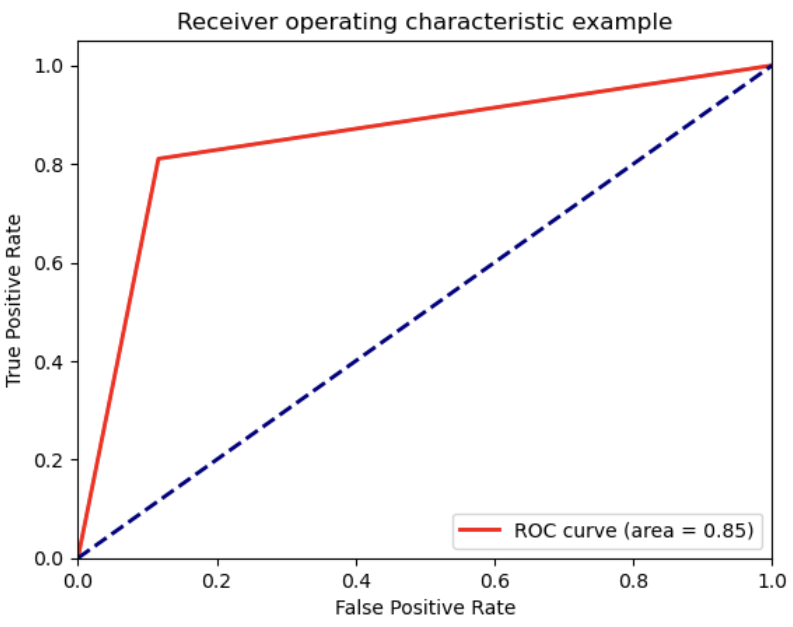
\includegraphics[width=0.75\textwidth]{roc.png}
	\caption{ROC Curve}
	\label{fig:roc}
\end{figure}

\newpage

\printbibliography

\end{document}
